\documentclass[english,t]{beamer}
%\documentclass[handout,english]{beamer}

\usepackage[T1]{fontenc}
\usepackage[utf8]{inputenc}
\usepackage{newtxtext} % times
%\usepackage[scaled=.95]{cabin} % sans serif
\usepackage{amsmath}
\usepackage[varqu,varl]{inconsolata} % typewriter
\usepackage[varg]{newtxmath}
\usefonttheme[onlymath]{serif} % beamer font theme
\usepackage{microtype}
\usepackage{afterpage}
\usepackage{url}
\urlstyle{same}
%\usepackage{amsbsy}
%\usepackage{eucal}
\usepackage{rotating}
%\usepackage{bm}
\usepackage{pdfpages}
\usepackage{algorithm}
\usepackage[noend]{algpseudocode}
\usepackage{booktabs}
\usepackage{listings}
\usepackage{lstbayes}
\graphicspath{{/home/ave/doc/images/}{}{../teranaloppu/}{../metodi/}{../slides/Hartikainen/}{../gphealth/}{../2008_09_RSS2008/}{../gphealth/}{../jyvaskyla2009/}{../nbbc2009/}{../gphealth/hippics/}{../euroheis2010/}{../pubgensens2011/}{../reykjavik2013/}{../liverpool2013/}{../../gpstuff/doc/}{./images/}{../aalto_stochastic/}{figs/}{../Stancon2018Helsinki/figs/}{../../paper/cvapprox/}{../gppa2017/}{../valencia2017/}{../../paper/combine_predictive_distribution/tex/}{../venice2018/figs/}{./figs/}}

% minted
\usepackage{minted}
\setminted{highlightcolor=yellow!25}
\newmintinline{r}{}
% The following is adjusted from
% https://tex.stackexchange.com/questions/548592/changing-all-colors-to-black-white-using-minted-sty
\makeatletter
\newcommand{\minted@style@bw}{%
  \renewcommand\fcolorbox[3][]{##3}%
  \renewcommand\textcolor[3][]{##3}%
  \color{gray}
}
% define new minted option "gray"
\minted@def@opt@switch{gray}
\fvset{formatcom*={%
  \ifthenelse{\equal{\minted@get@opt{gray}{true}}{true}}
  {\minted@style@bw}{}%
}}
\makeatother
% The following is ajusted from
% https://tex.stackexchange.com/questions/74459/remove-space-before-colorbox
\newcommand{\reducedstrut}{\vrule width 0pt height .9\ht\strutbox depth .9\dp\strutbox\relax}
\newcommand{\highlight}[1]{%
  \begingroup
  \setlength{\fboxsep}{0pt}%  
  \colorbox{yellow!30}{\reducedstrut\detokenize{#1}\/}%
  \endgroup
}

\usepackage{natbib}
\bibliographystyle{apalike}

\mode<presentation>
{
  \setbeamercovered{invisible}
  \setbeamertemplate{itemize items}[circle]
  \setbeamercolor{frametitle}{bg=white,fg=navyblue}
  \setbeamertemplate{navigation symbols}{}
  \setbeamertemplate{headline}[default]{}
  \setbeamertemplate{footline}[split]
  % \setbeamertemplate{headline}[text line]{\insertsection}
  \setbeamertemplate{footline}[frame number]
}

\pdfinfo{            
  /Title      (BDA, Lecture 8b) 
  /Author     (Aki Vehtari) % 
  /Keywords   (Bayesian data analysis)
}

%%%%%%%%%%%%%%%%%%% for tikz figures %%%%%%%%%%%%%%%%%%%%%%%%%%
\usepackage{ifthen}
\usepackage{tikz,pgfplots}
\usetikzlibrary{matrix}
\usetikzlibrary{calc}
\newlength{\figurewidth}
\newlength{\figureheight}

\newcommand*{\elpd}[2]{{\mathrm{elpd}\bigr(#1 \mid #2\bigl)}}
\newcommand*{\elpdHat}[2]{{\widehat{\mathrm{elpd}}_\mathrm{\scriptscriptstyle LOO}\bigr(#1 \mid #2\bigl)}}

\newcommand*{\elpdC}[2]{{\prescript{\mathrm{sv}}{}{} {\mathrm{elpd}\bigr(#1 \mid #2\bigl)}}}
\newcommand*{\Ma}{{\ensuremath{{\color{set12}\mathrm{M}_a}}}}
\newcommand*{\Mb}{{\ensuremath{{\color{set13}\mathrm{M}_b}}}}
\newcommand*{\Md}{{\ensuremath{{\color{set12}\mathrm{M}_a},{\color{set13}\mathrm{M}_b}}}}
%\newcommand*{\y}{\ensuremath{y}}
\newcommand*{\yobs}{\ensuremath{y^\text{obs}}}

\def\figpdfdir{./figs/} % directory for pdf-figures
\def\figtikzdir{./tikz/} % directory for tikz-figures 

% this is replacement for the \input command used in the figure-environment which
% takes into account whether pdf is forced
\newcommand{\minput}[2][]{
\ifthenelse{\equal{#1}{pdf}}
	{ \includegraphics{\figpdfdir #2} }
	{ \tikzset{external/remake next} \tikzsetnextfilename{#2} \input{\figtikzdir #2} }
}

% for externalization
\usetikzlibrary{external}
\tikzexternalize[prefix=\figpdfdir] 
\tikzset{external/system call={lualatex
	\tikzexternalcheckshellescape -halt-on-error -interaction=batchmode
	-jobname "\image" "\texsource"}}
    
%%%%%%%%%%%%%%%%%%% for hiding figures %%%%%%%%%%%%%%%%%%%%%%%%%%
\usepackage{color}
\newcommand{\hide}[5][white]{
	% usage: \hhide[color]{vspace,hspace,height,width}
	% note: all measures are relative units measured in \textwidth
	%\begin{minipage}{0.99\textwidth}
	\vspace{#2\textwidth}
	\hspace{#3\textwidth}
	\textcolor{#1}{  \rule{#5\textwidth}{#4\textwidth}  }
	% \end{minipage}
      }

\DeclareMathOperator{\Kfu}{\mathbf{K}_{f,u}}
\DeclareMathOperator{\Kuf}{\mathbf{K}_{u,f}}
\DeclareMathOperator{\Kff}{\mathbf{K}_{f,f}}
\DeclareMathOperator{\iKff}{\mathbf{K}_{f,f}^{-1}}
\DeclareMathOperator{\Kfa}{\mathbf{K}_{f,\tilde{f}}}
\DeclareMathOperator{\Kaf}{\mathbf{K}_{\tilde{f},f}}
\DeclareMathOperator{\Kaa}{\mathbf{K}_{\tilde{f},\tilde{f}}}
\DeclareMathOperator{\Kuu}{\mathbf{K}_{u,u}}
\DeclareMathOperator{\iKuu}{\mathbf{K}_{u,u}^{-1}}
\DeclareMathOperator{\Kau}{\mathbf{K}_{\tilde{f},u}}
\DeclareMathOperator{\Kua}{\mathbf{K}_{u,\tilde{f}}}
\DeclareMathOperator{\Qff}{\mathbf{Q}_{f,f}}
\DeclareMathOperator{\Qaa}{\mathbf{Q}_{\tilde{f},\tilde{f}}}
\DeclareMathOperator{\Qfa}{\mathbf{Q}_{f,\tilde{f}}}
\DeclareMathOperator{\Qaf}{\mathbf{Q}_{\tilde{f},f}}
\DeclareMathOperator{\x}{\mathbf{x}}
\DeclareMathOperator{\f}{\mathbf{f}}
\DeclareMathOperator{\y}{\mathbf{y}}
\DeclareMathOperator{\h}{\mathbf{h}}
\DeclareMathOperator{\uu}{\mathbf{u}}
\DeclareMathOperator{\LL}{\mathbf{\Lambda}}
\DeclareMathOperator{\bb}{\mathbf{b}}
\DeclareMathOperator{\E}{\mathrm{E}}
\def\WAIC{\mathrm{WAIC}}

\newcommand{\kin}{k^{\rm in}}
\newcommand{\kout}{k^{\rm out}}
\newcommand{\gi}{{R_0}}
\newcommand{\eff}{{E_{\rm max}}}
\newcommand{\HN}{{\rm N^+}}
\newcommand{\lN}{{\rm LN}}
\newcommand{\Rss}{R^{\rm ss}}
\newcommand{\invlogit}{\mbox{logit}^{-1}}

% \DeclareMathOperator{\Poisson}{Poisson}
\DeclareMathOperator{\Chi}{Chi}
\DeclareMathOperator{\GP}{\mathcal{GP}}
%\DeclareMathOperator{\N}{N}
\DeclareMathOperator{\normal}{normal}
\DeclareMathOperator{\KL}{KL}

\DeclareMathOperator*{\argmax}{arg\,max}
\DeclareMathOperator*{\argmin}{arg\,min}
\newcommand{\mb}{\mathbf}
\newcommand{\pkg}[1]{{\fontseries{b}\selectfont #1}}
\newcommand{\proglang}{}
\newcommand{\email}[1]{\href{mailto:#1}{\normalfont\texttt{#1}}}
\newcommand{\doi}[1]{\href{http://dx.doi.org/#1}{\normalfont\texttt{doi:#1}}}
\newcommand{\code}[1]{{\normalfont\texttt{#1}}}

% \DeclareMathOperator{\E}{E}
\DeclareMathOperator{\Var}{Var}
\DeclareMathOperator{\var}{var}
\DeclareMathOperator{\cov}{cov}
\DeclareMathOperator{\logistic}{logistic}
\DeclareMathOperator{\softmax}{softmax}
\DeclareMathOperator{\Multinomial}{Multinomial}
\DeclareMathOperator{\Sd}{Sd}
\DeclareMathOperator{\sd}{sd}
\DeclareMathOperator{\Bin}{Bin}
\DeclareMathOperator{\Poisson}{Poisson}
\DeclareMathOperator{\Beta}{Beta}
\DeclareMathOperator{\logit}{logit}
\DeclareMathOperator{\N}{N}
\DeclareMathOperator{\U}{U}
\DeclareMathOperator{\BF}{BF}
%\DeclareMathOperator{\Pr}{Pr}
\def\euro{{\footnotesize \EUR\, }}
\DeclareMathOperator{\rep}{\mathrm{rep}}

\definecolor{set11}{HTML}{E41A1C}
\definecolor{set12}{HTML}{377EB8}
\definecolor{set13}{HTML}{4DAF4A}
\definecolor{greenish}{rgb}{0.1333,0.8666,0.1333}
\definecolor{forestgreen}{rgb}{0.1333,0.5451,0.1333}
\definecolor{darkgreen}{rgb}{0,0.5,0}
\definecolor{hutblue}{rgb}{0,0.2549,0.6784}
\definecolor{midnightblue}{rgb}{0.0977,0.0977,0.4375}
\definecolor{navyblue}{rgb}{0,0,0.5}
\definecolor{hutsilver}{rgb}{0.4863,0.4784,0.4784}
\definecolor{lightgray}{rgb}{0.95,0.95,0.95}
\definecolor{section}{rgb}{0,0.2549,0.6784}
\definecolor{list1}{rgb}{0,0.2549,0.6784}
\renewcommand{\emph}[1]{\textcolor{navyblue}{#1}}


\parindent=0pt
\parskip=8pt
\tolerance=9000
\abovedisplayshortskip=0pt

% Lists
\newenvironment{list1}{
   \begin{list}{$\color{list1}\bullet$}{\itemsep=6pt}}{
  \end{list}}
\newenvironment{list1s}{
  \begin{list}{$\includegraphics[width=5pt]{logo.eps}$}{\itemsep=6pt}}{
  \end{list}}
\newenvironment{list2}{
  \begin{list}{-}{\baselineskip=12pt\itemsep=2pt}}{
  \end{list}}
\newenvironment{list3}{
  \begin{list}{$\cdot$}{\baselineskip=15pt}}{
  \end{list}}

\title[]{Bayesian data analysis}
\subtitle{}

\author{Aki Vehtari}

\institute[Aalto]{}
 
\date[]{}

%\beamerdefaultoverlayspecification{<+->}

\begin{document}
 
\begin{frame}{Predicting concrete quality}

  \only<1>{
      \hspace{-6mm}
    \begin{minipage}[c]{0.475\linewidth}
    \includegraphics[height=3.7cm,trim=200 0 254 0,clip]{45396382385_3aa7f81768_k_ccby.jpg}
    \end{minipage}
    \begin{minipage}[c]{0.8cm}
      \centering
      \hspace{3mm}$\rightarrow$\hspace{-1.5mm}
    \end{minipage}
    \begin{minipage}[c]{0.475\linewidth}
    \includegraphics[height=3.7cm]{ConcreteBridge.jpg}
    \end{minipage}
    }
  % \begin{center}
  %   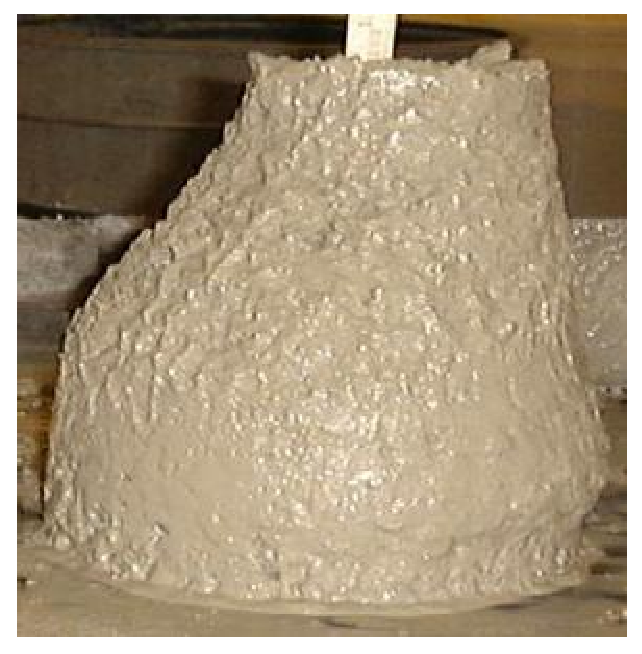
\includegraphics[width=5cm]{slump1b.eps}
  % \end{center}

    \begin{itemize}
    \item How accurate the model is?
    \item Is it better than predicting with random guess?
    \item Is it possible that the model has overfitted?
    \item Is model B better than model A?
    \end{itemize}
\end{frame}

\begin{frame}{Outline}

  \vspace{-.5\baselineskip}
  \begin{itemize}
  \item What is cross-validation
  \begin{list2}
    \item Leave-one-out cross-validation (elpd\_loo, p\_loo)
    \item Uncertainty in LOO (SE)
    \end{list2}
  \item Fast cross-validation
    \begin{list2}
    \item PSIS and diagnostics in loo package (Pareto k, n\_eff, Monte Carlo SE)
    \end{list2}
  \item Model comparison and selection (elpd\_diff, se)
  \end{itemize}
    {\color{gray}
Next week
  \begin{itemize}
    \color{gray}
  \item When is cross-validation applicable?
    \begin{list2}
    \item data generating mechanisms and prediction tasks
    \item leave-many-out cross-validation
    \end{list2}
  \item $K$-fold cross-validation
  \item {\footnotesize Related methods (WAIC, *IC, BF)}
  \item Model averaging
  \item Hypothesis testing
  \item Potential overfitting in model selection
  % \item<2-> Part 2: Projective Inference in High-dimensional Problems:
  %   Prediction and Feature Selection
  \end{itemize}
}

\end{frame}

\begin{frame}{Chapter 7}

  \vspace{-\baselineskip}
   \begin{itemize}
   \item 7.1 Measures of predictive accuracy
   \item {\color{gray} 7.2 Information criteria and cross-validation}
     \begin{list2}
     \item Instead of 7.2, read:\\
       Vehtari, A., Gelman, A., Gabry, J. (2017). Practical Bayesian
       model evaluation using leave-one-out cross-validation and
       WAIC. Statistics and Computing. 27(5):1413–1432.
       \href{http://arxiv.org/abs/1507.04544}{preprint at arxiv.org/abs/1507.04544}.
     \item See also \url{https://users.aalto.fi/~ave/modelselection/CV-FAQ.html}

     \end{list2}
     \end{itemize}
Next week
   \begin{itemize}
   \item 7.3 Model comparison based on predictive performance\\
   \item 7.4 Model comparison using Bayes factors\\
   \item 7.5 Continuous model expansion / sensitivity analysis
   \item {\color{gray}7.5 Example (may be skipped)}
   \end{itemize}

\end{frame}

% \begin{frame}{Model assessment, selection and inference after selection}

%    \begin{list1}
%    \item Extra material at \url{https://users.aalto.fi/~ave/modelselection/}
%      \begin{list2}
%        % \item Videos, Slides, Notebooks, References
%        % \item The most relevant for the course is the first part of the
%        %   talk ``Model assessment, comparison and selection at Master
%        %   class in Bayesian statistics, CIRM, Marseille''
%      \end{list2}
%    \end{list1}

% \end{frame}
% \begin{frame}{Predicting cancer recurrence}

%   \begin{center}
%     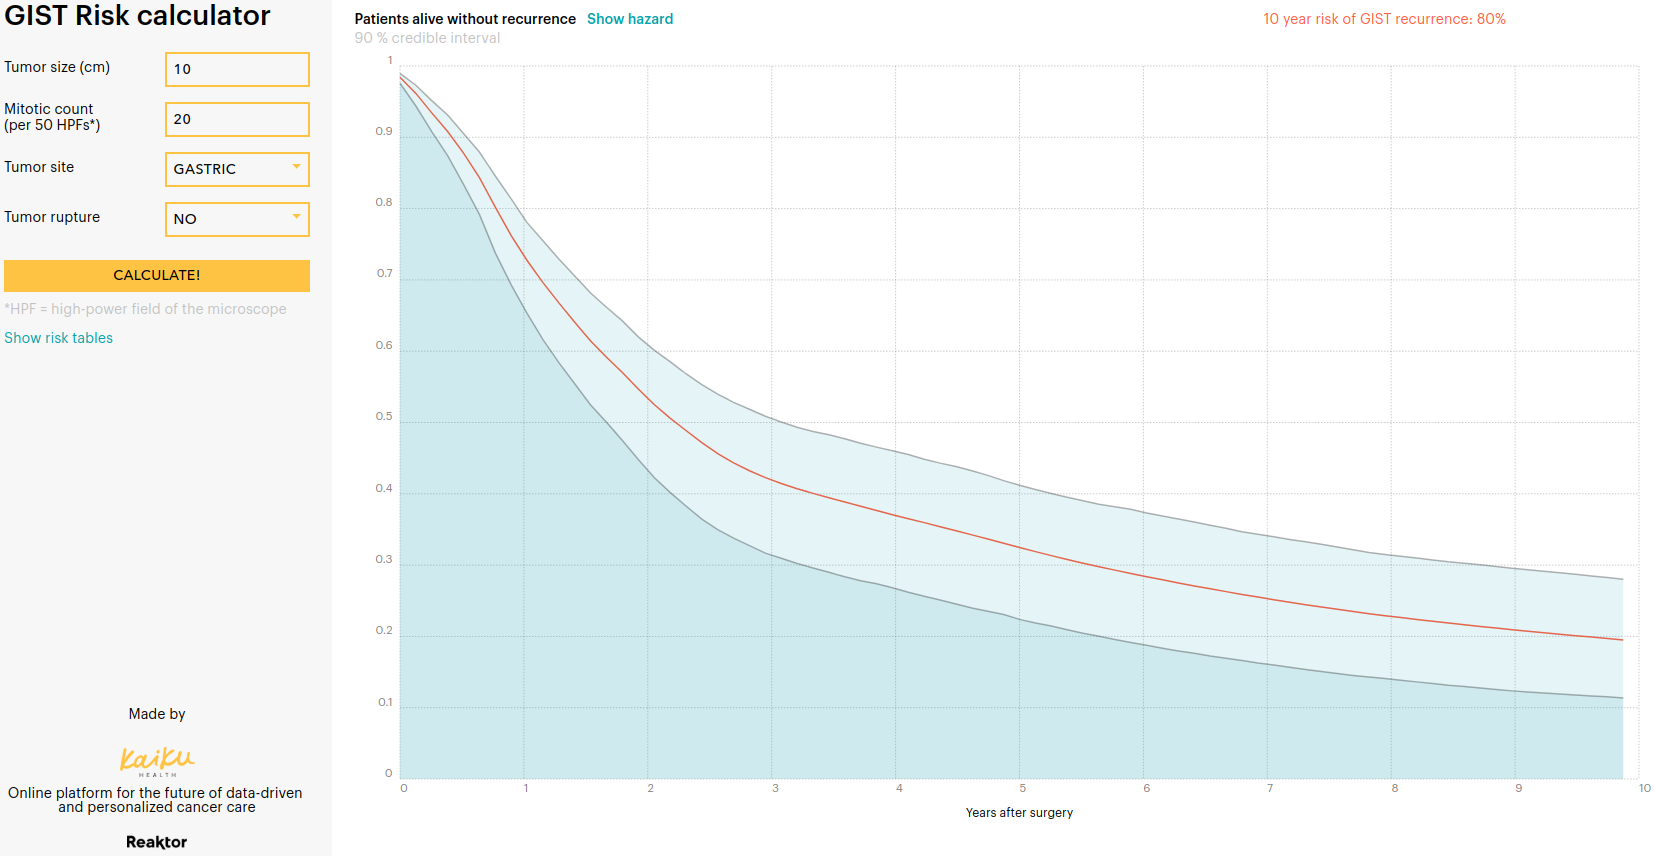
\includegraphics[width=11.5cm]{gistrisk.png}
%   \end{center}
  
% \end{frame}

\begin{frame}{Predictive performance}

  \begin{itemize}
  \item<1-> True predictive performance is found out by using it to make
    predictions and comparing predictions to true observations
    \begin{itemize}
      \item external validation
    \end{itemize}
  \item<2-> Expected predictive performance
    \begin{itemize}
      \item approximates the external validation
      \end{itemize}
    \end{itemize}

\end{frame}

% \begin{frame}{}

%   {\Large\color{navyblue} Model assessment, comparison, selection and averaging}

%   \begin{list1}
%   \item Modeling complex phenomena with models that
%     are much simpler than the nature ($M$-open)
%   \item<2-> Decision theoretical approch in spirit of
%     \begin{list2}
%     \item Lindley, Box, Rubin, Bernardo \& Smith, etc.
%     \end{list2}
%   \end{list1}
  
% \end{frame}

\begin{frame}{Predictive performance}

  \begin{itemize}
  \item We need to choose the utility/cost function
    \begin{itemize}
    \item more about these in lecture 10
    \end{itemize}
  \item Application specific utility/cost functions are important
    \begin{itemize}
      \item eg. money, life years, quality adjusted life years, etc.
    \end{itemize}
    \pause
  \item If we are interested overall in the goodness of the predictive distribution,
    or we don't know (yet) the application specific utility, then
    good information theoretically justified choice is log-score
      \begin{align*}
        \log p(y^{\text{rep}}  \mid  y, M),
      \end{align*}
\end{itemize}

\end{frame}

\begin{frame}[fragile]
  \frametitle{Stan and {\tt loo} package}

  \vspace{-\baselineskip}
  Model assessment:
  \vspace{-0.5\baselineskip}
\begin{minted}[fontsize=\scriptsize]{text}
Computed from 4000 by 20 log-likelihood matrix

         Estimate  SE
elpd_loo    -29.5 3.3
p_loo         2.7 1.0
------
------
MCSE of elpd_loo is 0.1.
MCSE and ESS estimates assume MCMC draws (r_eff in [0.6, 1.2]).

All Pareto k estimates are good (k < 0.7).
See help('pareto-k-diagnostic') for details.
\end{minted}
Model comparison:
  \vspace{-0.5\baselineskip}
\begin{minted}[fontsize=\scriptsize]{text}
(negative 'elpd_diff' favors 1st model, positive favors 2nd) 

elpd_diff        se 
     -0.2       0.1 
\end{minted}

\end{frame}


\begin{frame}{}

  \only<1>{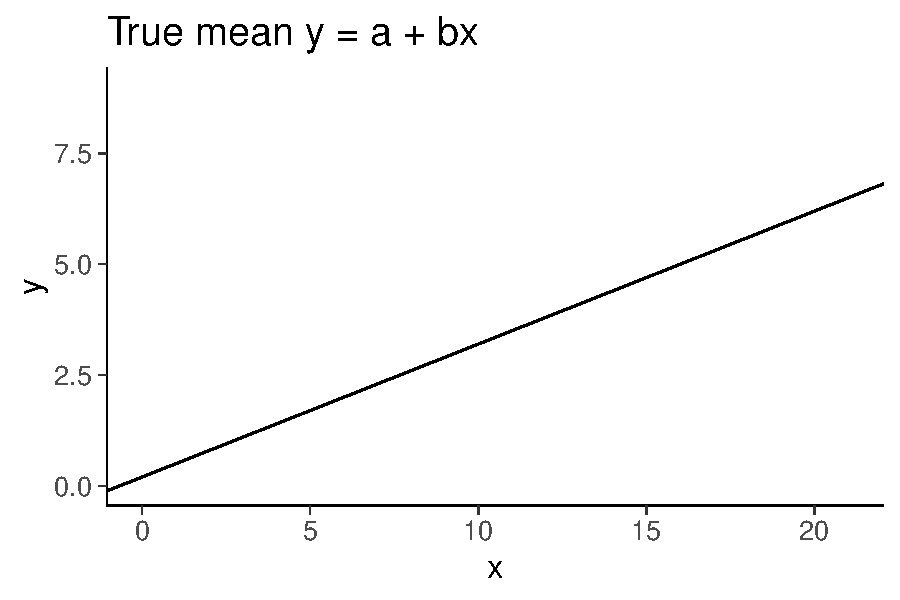
\includegraphics[width=10cm]{fake1.pdf}}
  \only<2>{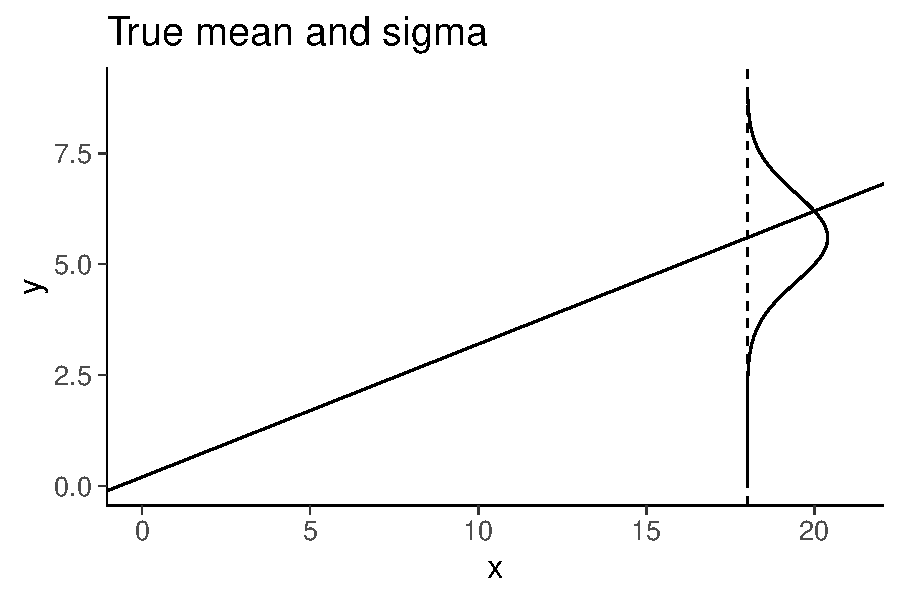
\includegraphics[width=10cm]{fake2.pdf}}
  \only<3>{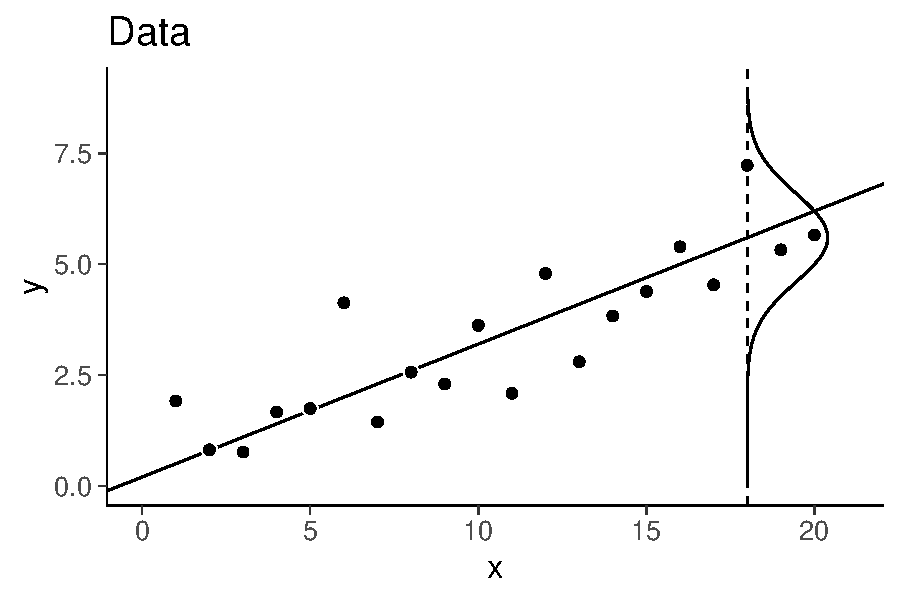
\includegraphics[width=10cm]{fake3.pdf}}
  \only<4>{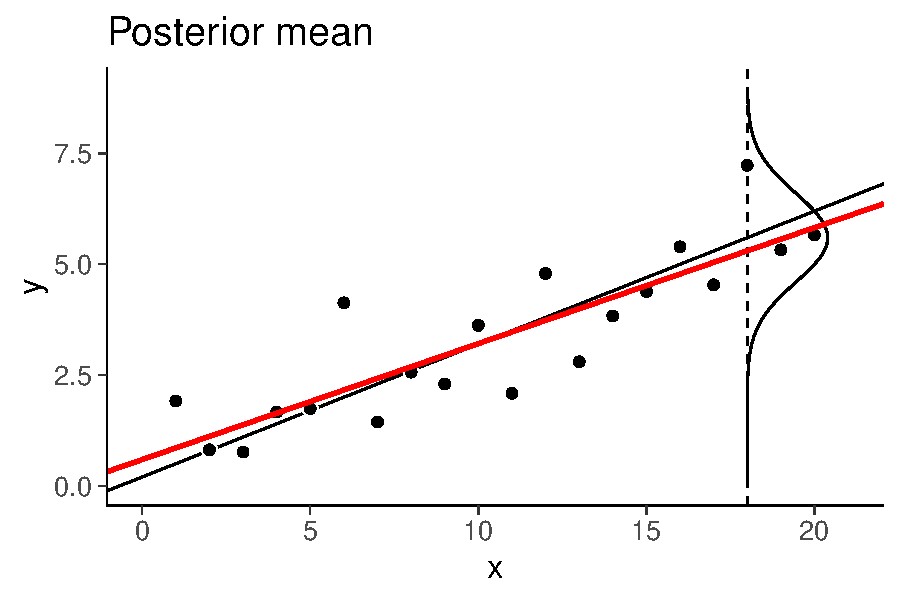
\includegraphics[width=10cm]{fake4.pdf}}
  \only<5>{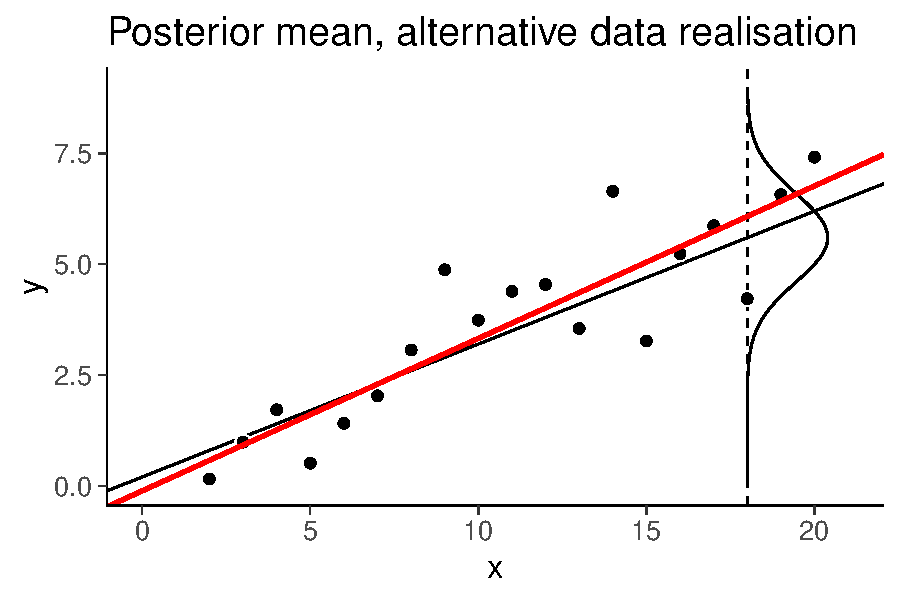
\includegraphics[width=10cm]{fake4b.pdf}}
  \only<6>{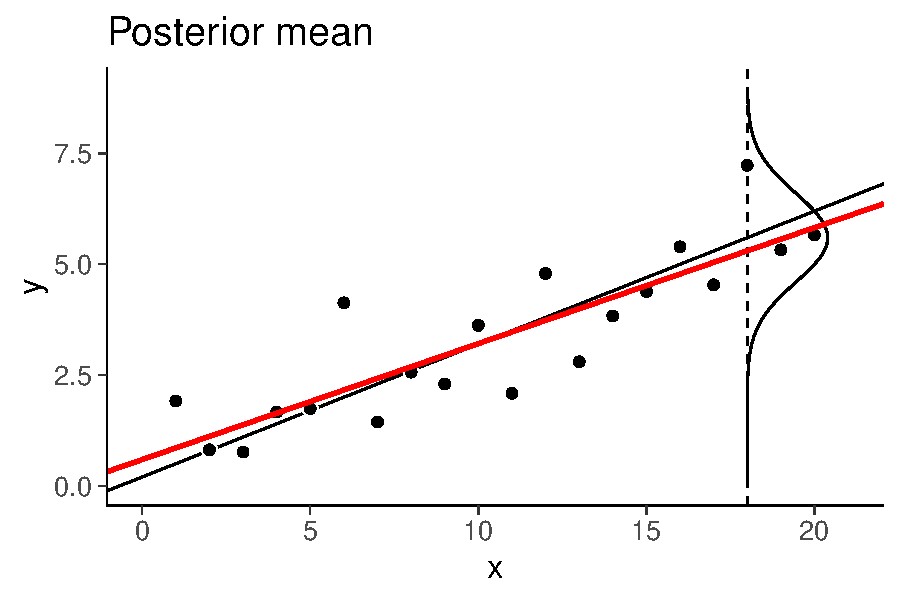
\includegraphics[width=10cm]{fake4.pdf}}
  \only<7>{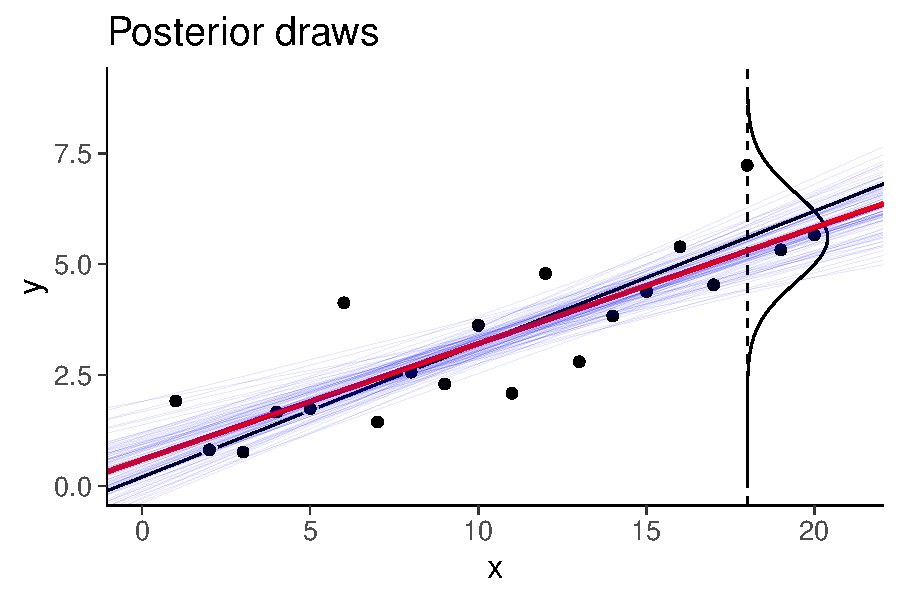
\includegraphics[width=10cm]{fake4s.pdf}}
  \only<8-9>{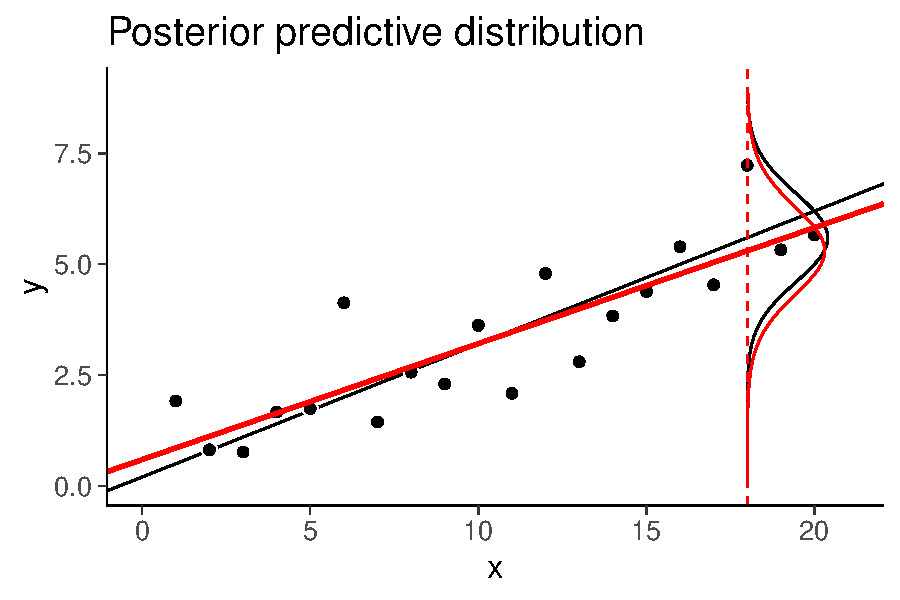
\includegraphics[width=10cm]{fake5.pdf}}
  \only<10>{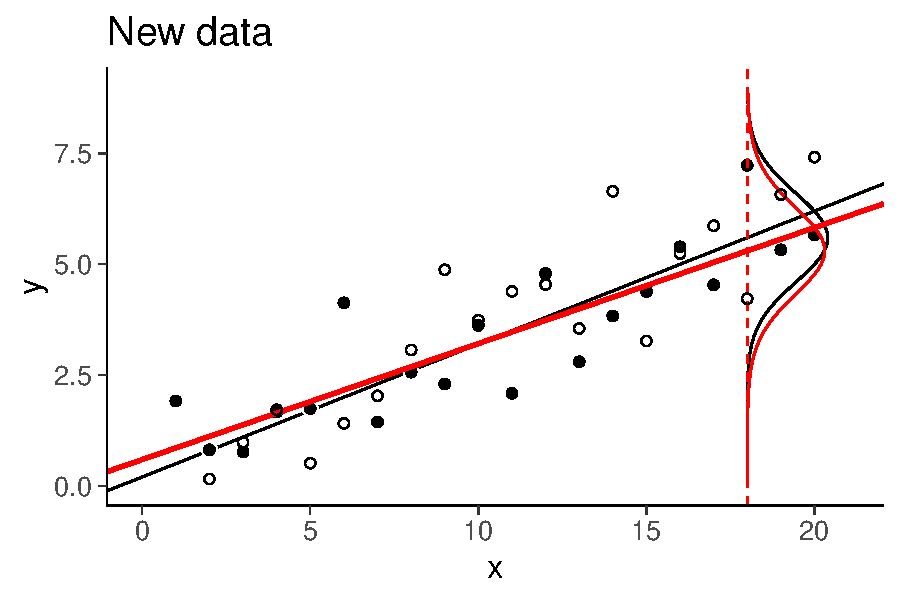
\includegraphics[width=10cm]{fake5n.pdf}}
  \only<11>{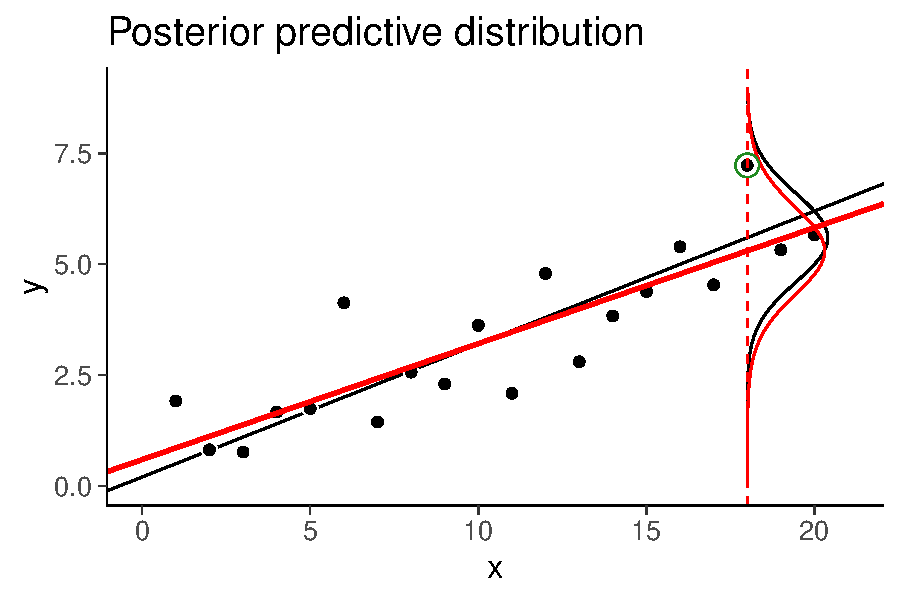
\includegraphics[width=10cm]{fake6.pdf}}
  \only<12>{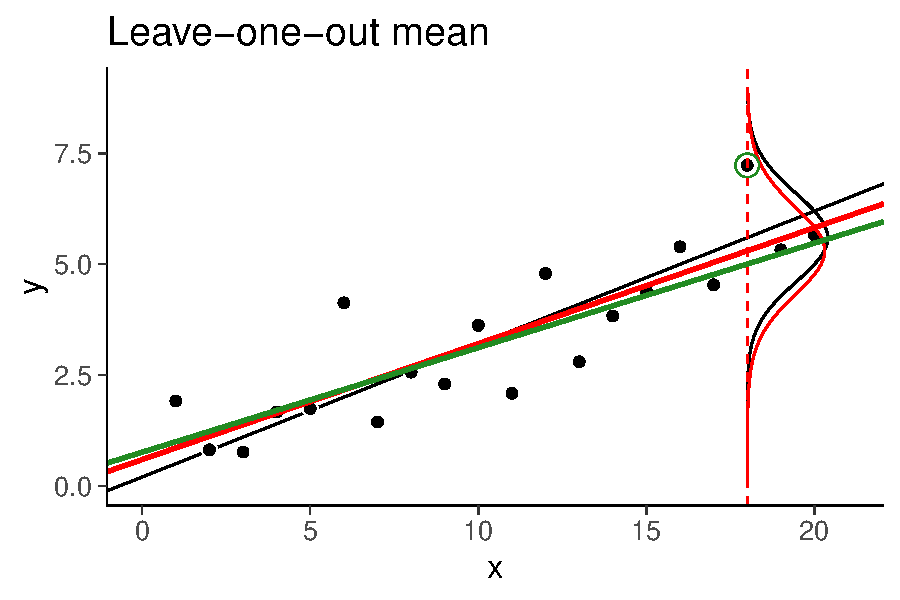
\includegraphics[width=10cm]{fake7.pdf}}
  \\
  \onslide<9>{\color{red} $p(\tilde{y} \mid \tilde{x}=18,x,y)=\int p(\tilde{y} \mid \tilde{x}=18,\theta)p(\theta \mid x,y)d\theta$\\ \vspace{0.5\baselineskip}}
\end{frame}

\begin{frame}{}

  {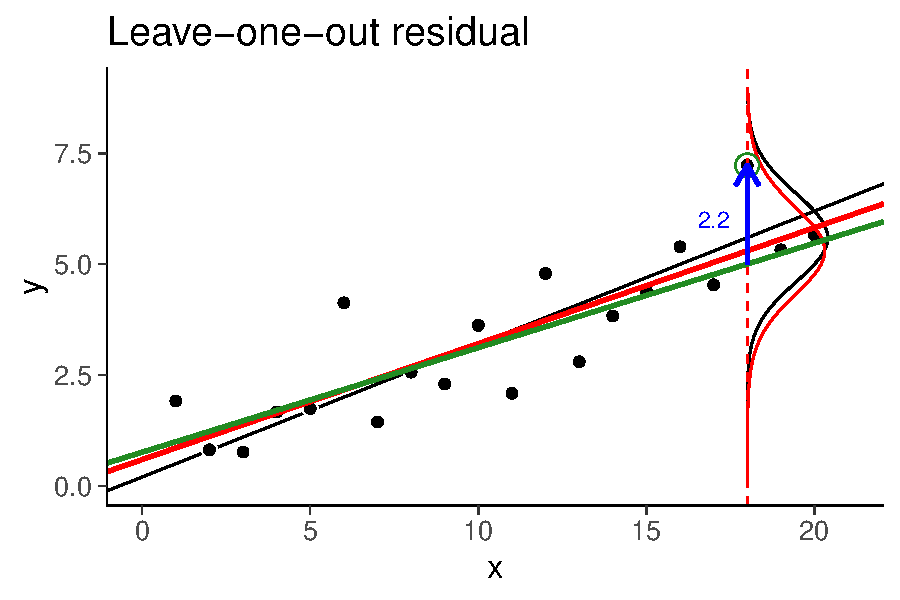
\includegraphics[width=10cm]{fake7r.pdf}}
  \\
  \onslide<2->{{\color{blue} $y_{18} - E[p(\tilde{y} \mid \tilde{x}=18,x_{-18},y_{-18})]$}\\\vspace{0.5\baselineskip}}
  \onslide<3->{Can be used to compute, e.g., RMSE, $R^2$, 90\% error}
  \onslide<4>{\\~\\ \small See LOO-$R^2$ at \url{avehtari.github.io/bayes_R2/bayes_R2.html}}
\end{frame}

\begin{frame}{}

  {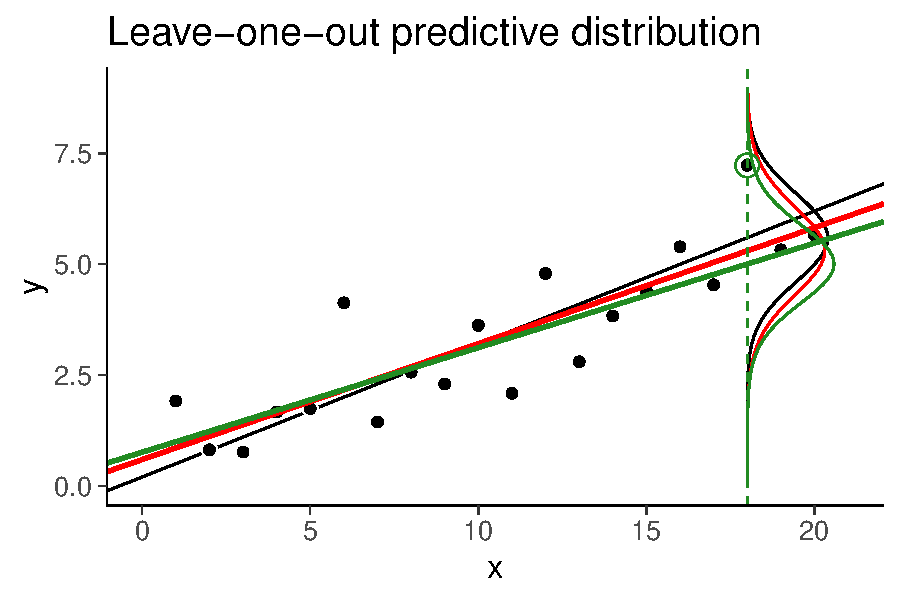
\includegraphics[width=10cm]{fake8.pdf}}
  \\
  \onslide<2>{\color{forestgreen}$p(\tilde{y} \mid \tilde{x}=18,x_{-18},y_{-18})=\int p(\tilde{y} \mid \tilde{x}=18,\theta)p(\theta \mid x_{-18},y_{-18})d\theta$}
  
\end{frame}

\begin{frame}{}

  \only<1-2>{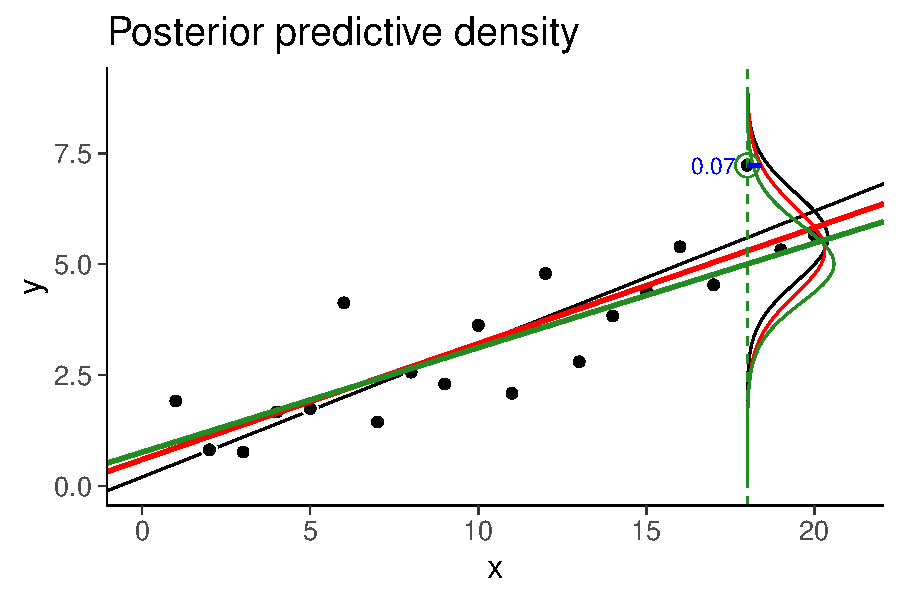
\includegraphics[width=10cm]{fake8pd.pdf}}
  \only<3>{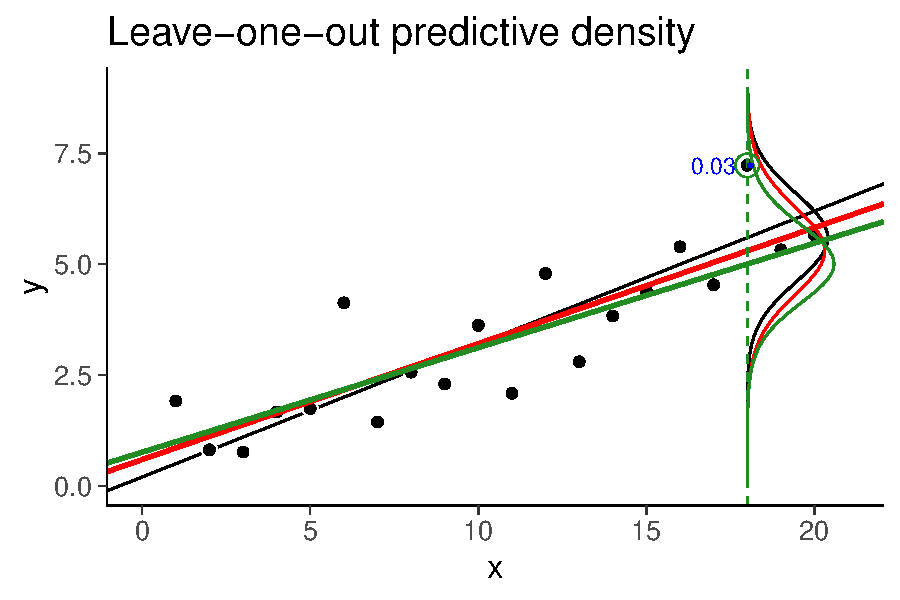
\includegraphics[width=10cm]{fake8loopd.pdf}}
  \\
  \onslide<2->{\color{red} $p(\tilde{y}=y_{18} \mid \tilde{x}=18,x,y) \approx 0.07$\\ \vspace{0.5\baselineskip}}
  \onslide<3>{\color{forestgreen} $p(\tilde{y}=y_{18} \mid \tilde{x}=18,x_{-18},y_{-18}) \approx 0.03$}
  
\end{frame}

\begin{frame}{}

  \only<1>{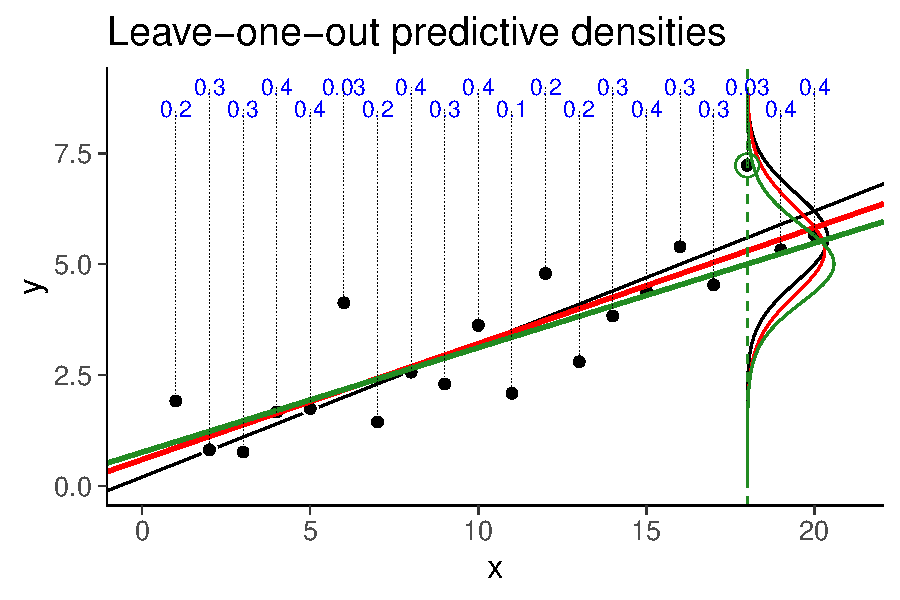
\includegraphics[width=10cm]{fake8loopds.pdf}}
  \only<2->{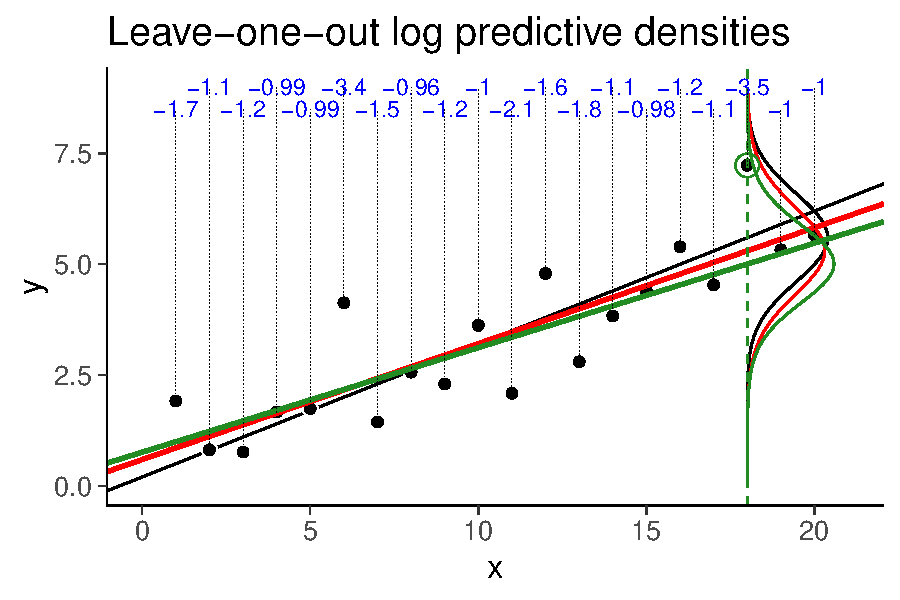
\includegraphics[width=10cm]{fake8loolpds.pdf}}
  \\ \vspace{-\baselineskip}\\
  \only<1>{\color{blue} $p(y_i \mid x_i,x_{-i},y_{-i}), \quad i=1,\ldots,20$}
  \only<2>{\color{blue} $\log p(y_i \mid x_i,x_{-i},y_{-i}), \quad i=1,\ldots,20$}
  \only<3>{\color{blue} $\sum_{i=1}^{20} \log p(y_i \mid x_i,x_{-i},y_{-i}) \approx -29.5$}
  \only<4->{\color{blue} $\mbox{elpd\_loo} = \sum_{i=1}^{20} \log p(y_i \mid x_i,x_{-i},y_{-i}) \approx -29.5$\\ \vspace{0.5\baselineskip}}
  \only<5> {{\color{blue}an estimate of log posterior pred. density for new data}}
  \only<6-7>{\color{red}$\mbox{lpd} = \sum_{i=1}^{20} \log p(y_i \mid x_i,x,y) \approx -26.8$\\ \vspace{0.2\baselineskip}}
  \only<7->{\color{blue} $\mbox{p\_loo} = \mbox{lpd}-\mbox{elpd\_loo} \approx 2.7$\\}
  \only<8->{{\color{black}asymptotically approaches $p$ in case of regular faithful model}}
  \only<9>{\vfill \color{black} \footnotesize see \href{http://link.springer.com/article/10.1007/s11222-016-9696-4}{Vehtari, Gelman \& Gabry (2017a)} and \href{http://dx.doi.org/10.1214/12-SS102}{Vehtari \& Ojanen (2012)} for more}
  
\end{frame}

\begin{frame}{}

  {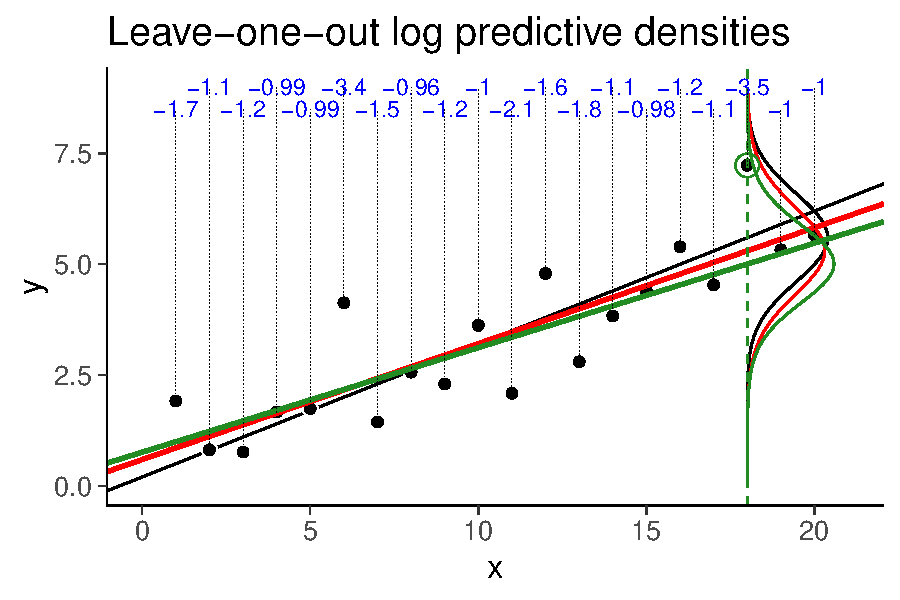
\includegraphics[width=10cm]{fake8loolpds.pdf}}\\
  \vspace{-\baselineskip}\\
  {\color{blue} $\mbox{elpd\_loo} = \sum_{i=1}^{20} \log p(y_i \mid x_i,x_{-i},y_{-i}) \approx -29.5$\\ \vspace{0.5\baselineskip}}
  {\color{blue} $\mbox{SE} = \sd(\log p(y_i \mid x_i,x_{-i},y_{-i}))\cdot \sqrt{20} \approx 3.3$}
  {\vfill \color{black} \footnotesize see \href{http://link.springer.com/article/10.1007/s11222-016-9696-4}{Vehtari, Gelman \& Gabry (2017a)} and \href{http://dx.doi.org/10.1214/12-SS102}{Vehtari \& Ojanen (2012)} for more}
  
\end{frame}

\begin{frame}[fragile]{{\tt loo} package}

\begin{minted}[fontsize=\footnotesize]{text}
Computed from 4000 by 20 log-likelihood matrix

         Estimate  SE
elpd_loo    -29.5 3.3
p_loo         2.7 1.0
\end{minted}
      {\color{gray}
\begin{minted}[fontsize=\footnotesize]{text}
------
MCSE of elpd_loo is 0.1.
MCSE and ESS estimates assume MCMC draws (r_eff in [0.6, 1.0]).

All Pareto k estimates are good (k < 0.7).
See help('pareto-k-diagnostic') for details.
\end{minted}
      }

\end{frame}

\begin{frame}[fragile]{Helicopter flight time -- elpd}

\begin{minted}[fontsize=\footnotesize]{text}
Computed from 4000 by 150 log-likelihood matrix.

         Estimate   SE
elpd_loo    -79.2  9.9
p_loo         8.3  1.4
\end{minted}
{\color{gray}
\begin{minted}[fontsize=\footnotesize]{text}
------
MCSE of elpd_loo is 0.1.
MCSE and ESS estimates assume MCMC draws (r_eff in [0.6, 1.2]).

All Pareto k estimates are good (k < 0.7).
See help('pareto-k-diagnostic') for details.
\end{minted}
}

\end{frame}

\begin{frame}[fragile]{Helicopter flight time -- $R^2$}

$R^2$ is the proportion of variance explained by the model

\begin{minted}[fontsize=\footnotesize]{text}
> bayes_R2(fit) |> round(digits=2)
   Estimate Est.Error Q2.5 Q97.5
R2     0.51      0.04 0.42  0.58

> loo_R2(fit) |> round(digits=2)
   Estimate Est.Error Q2.5 Q97.5
R2     0.47      0.06 0.35  0.57
\end{minted}

\end{frame}

\begin{frame}[fragile]{Student retention -- $R^2$}

$R^2$ is the proportion of variance explained by the model
  
\begin{minted}[fontsize=\footnotesize]{text}
> bayes_R2(fit6) |> round(digits=2)
   Estimate Est.Error Q2.5 Q97.5
R2     0.98         0 0.97  0.98

> loo_R2(fit6) |> round(digits=2)
   Estimate Est.Error Q2.5 Q97.5
R2     0.97      0.01 0.95  0.98
\end{minted}

\end{frame}

\begin{frame}[fragile]{Student retention}
%\framesubtitle{\texttt{pp\_check(fit, type = "intervals\_grouped", group="year")}}

\vspace{-0.8\baselineskip}  
Posterior predictive intervals\\  
  \hspace{-7mm}
  \begin{minipage}[t][3.6cm][t]{1.0\linewidth}
    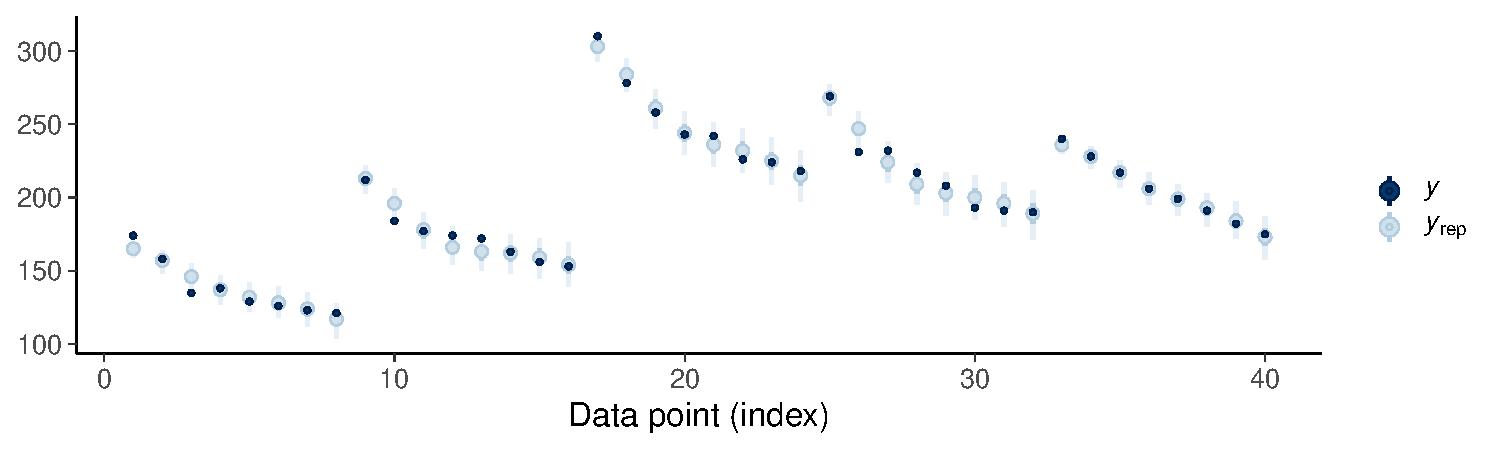
\includegraphics[height=3.6cm]{student_retention_sbinom_ppc_intervals.pdf}
  \end{minipage}
  
\vspace{-0.5\baselineskip}  
LOO predictive intervals\\  
  \hspace{-7mm}
  \begin{minipage}[t][3.6cm][t]{1.0\linewidth}
    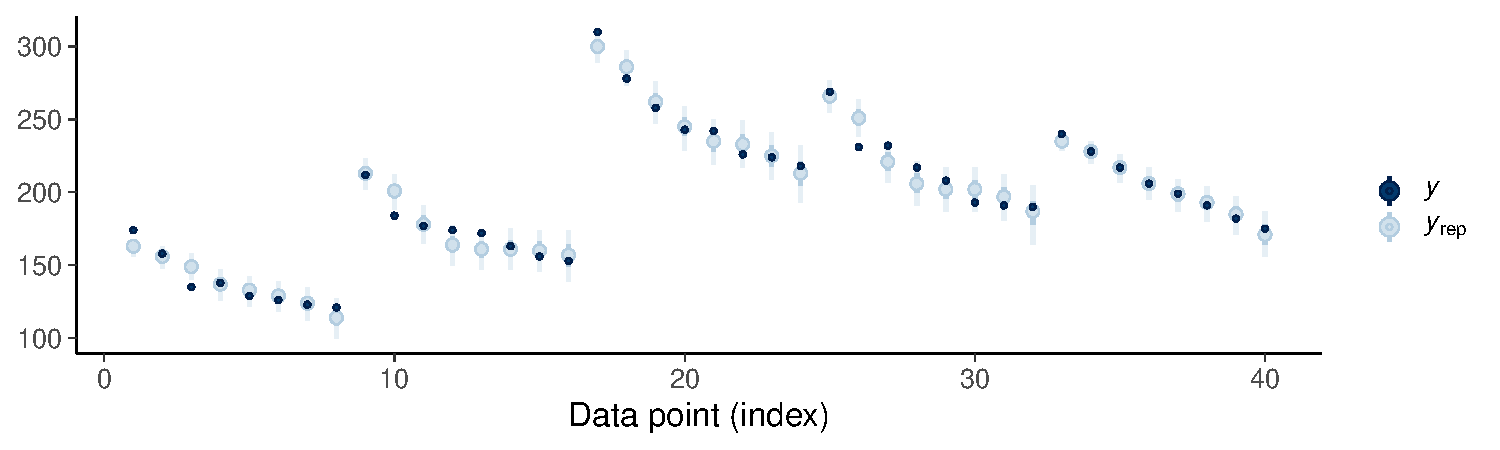
\includegraphics[height=3.6cm]{student_retention_sbinom_ppc_loo_intervals.pdf}
  \end{minipage}  

\end{frame}

\begin{frame}[fragile]{Student retention -- $R^2$}

Latent hierarchical linear vs. latent hierarchical linear + spline
  
\begin{minted}[fontsize=\footnotesize]{text}
> loo_R2(fit4) |> round(digits=2)
   Estimate Est.Error Q2.5 Q97.5
R2     0.92      0.02 0.88  0.95

> loo_R2(fit6) |> round(digits=2)
   Estimate Est.Error Q2.5 Q97.5
R2     0.97      0.01 0.95  0.98
\end{minted}

\end{frame}

\begin{frame}[fragile]{Student retention -- elpd (log score)}

Latent hierarchical linear vs. latent hierarchical linear + spline
  
\begin{minted}[fontsize=\footnotesize]{text}
> loo_compare(fit4, fit6)
     elpd_diff se_diff
fit6   0.0       0.0  
fit4 -43.2      14.4  
\end{minted}

More about this soon
  
\end{frame}

\begin{frame}{LOO-PIT predictive checking}

  \vspace{-0.5\baselineskip}
  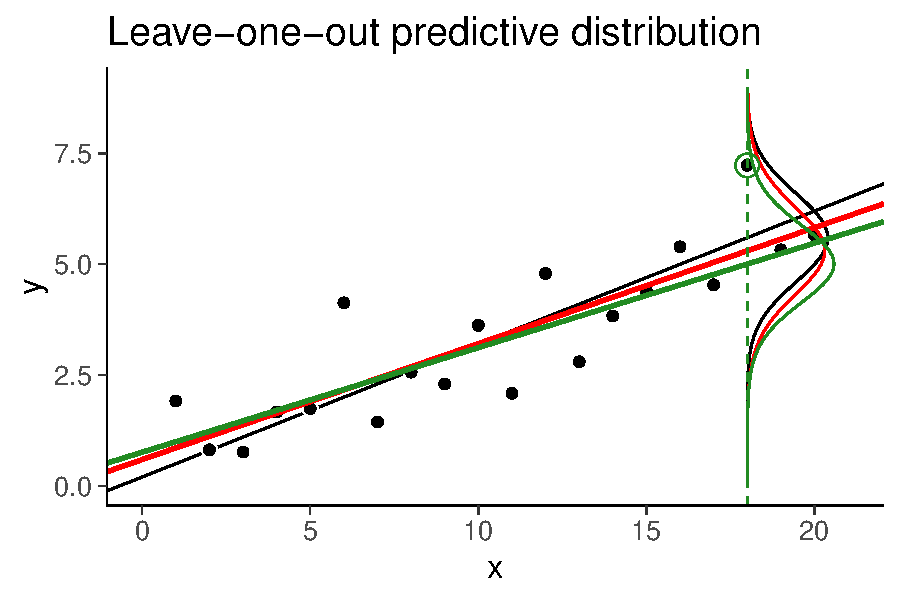
\includegraphics[width=9cm,trim=0 0 0 30,clip]{fake8.pdf}
  
  \vspace{-0.5\baselineskip}
  \begin{itemize}
  \item LOO probability integral transform (LOO-PIT)
    \begin{align*}
      p_i = p(y_i^{\rep} \leq y_i | y_{-i})
    \end{align*}
  \item If $p(\tilde{y}_i|y_{-i})$ is well calibrated, distribution of $p_i$'s
    would be uniform between 0 and 1
  \end{itemize}

\end{frame}

\begin{frame}[fragile]{Student retention -- LOO-PIT checking}
\framesubtitle{\texttt{pp\_check(fit, type = "loo\_pit\_qq", ndraws=4000)}}

\vspace{-0.5\baselineskip}  
Latent hierarchical linear -- LOO predictive intervals\\  
  \hspace{-7mm}
  \begin{minipage}[t][3.6cm][t]{1.0\linewidth}
    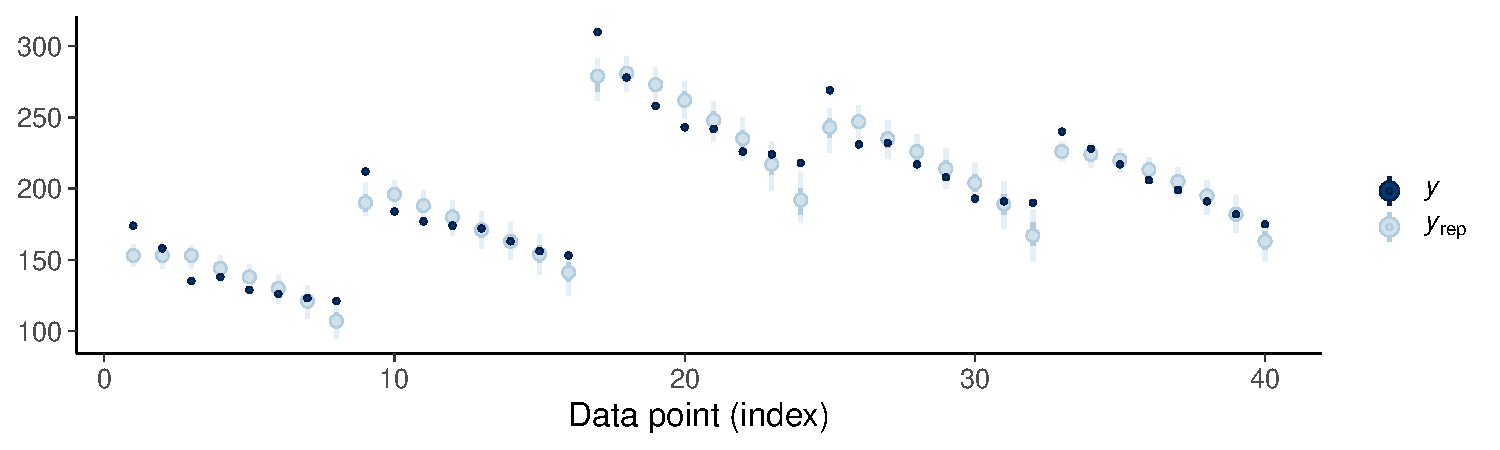
\includegraphics[height=3.6cm]{student_retention_lbinom_ppc_loo_intervals.pdf}
  \end{minipage}  

\vspace{-0.5\baselineskip}  
LOO-PIT check\\  
  \hspace{-7mm}
  \begin{minipage}[t][3.6cm][t]{1.0\linewidth}
    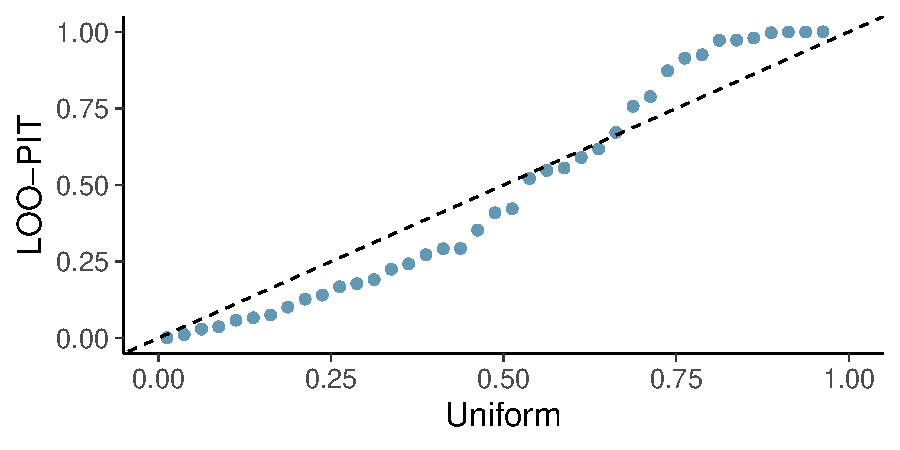
\includegraphics[height=3.6cm]{student_retention_lbinom_ppc_loo_pit_qq.pdf}
  \end{minipage}  

\end{frame}

\begin{frame}[fragile]{Student retention -- LOO-PIT checking}
\framesubtitle{\texttt{pp\_check(fit, type = "loo\_pit\_qq", ndraws=4000)}}

\vspace{-0.5\baselineskip}  
Latent hierarchical linear + spline -- LOO predictive intervals/\\  
  \hspace{-7mm}
  \begin{minipage}[t][3.6cm][t]{1.0\linewidth}
    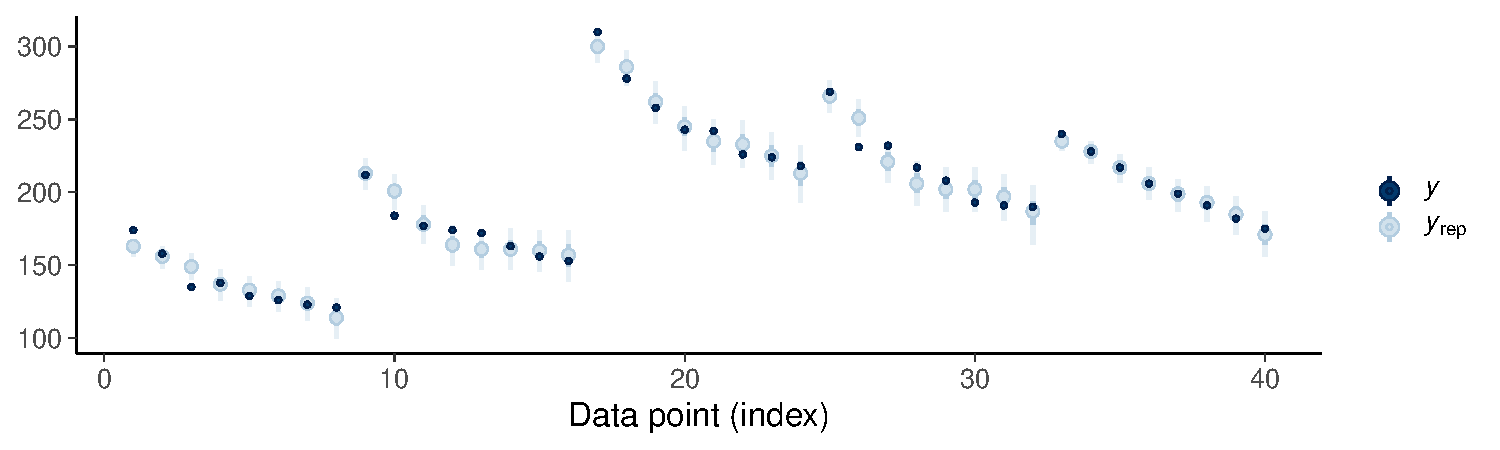
\includegraphics[height=3.6cm]{student_retention_sbinom_ppc_loo_intervals.pdf}
  \end{minipage}  

\vspace{-0.5\baselineskip}  
LOO-PIT check\\  
  \hspace{-7mm}
  \begin{minipage}[t][3.6cm][t]{1.0\linewidth}
    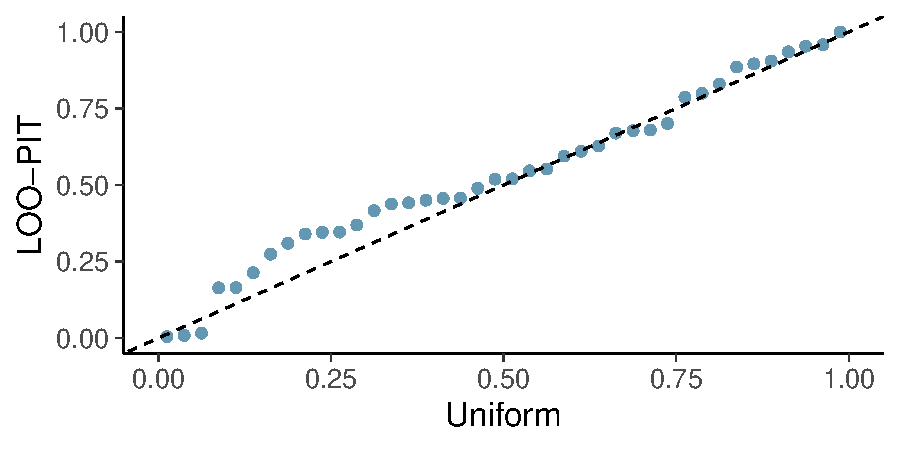
\includegraphics[height=3.6cm]{student_retention_sbinom_ppc_loo_pit_qq.pdf}
  \end{minipage}  

\end{frame}

% \begin{frame}{Example: Exposure to air pollution}

%   LOO predictive checking -- LOO-PIT

% 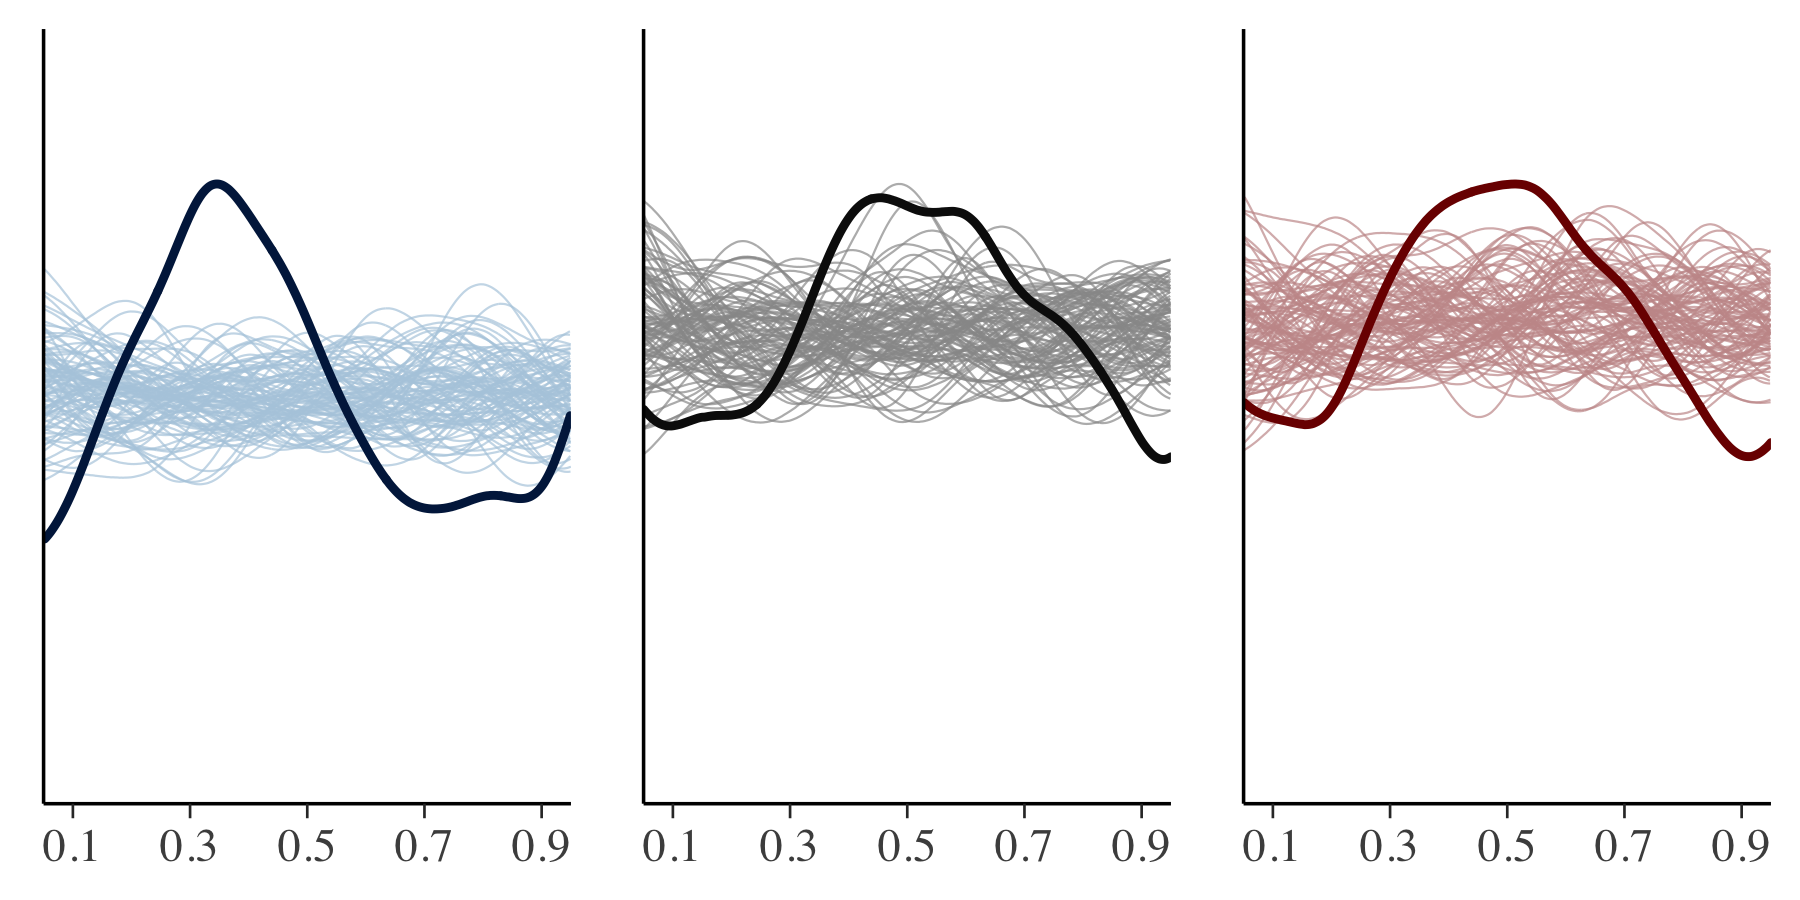
\includegraphics[width=\textwidth]{ppc_loo_pit_corrected_pm25.png}

% % \begin{figure}
% % \centering
% % \begin{subfigure}{0.31\textwidth}
% % 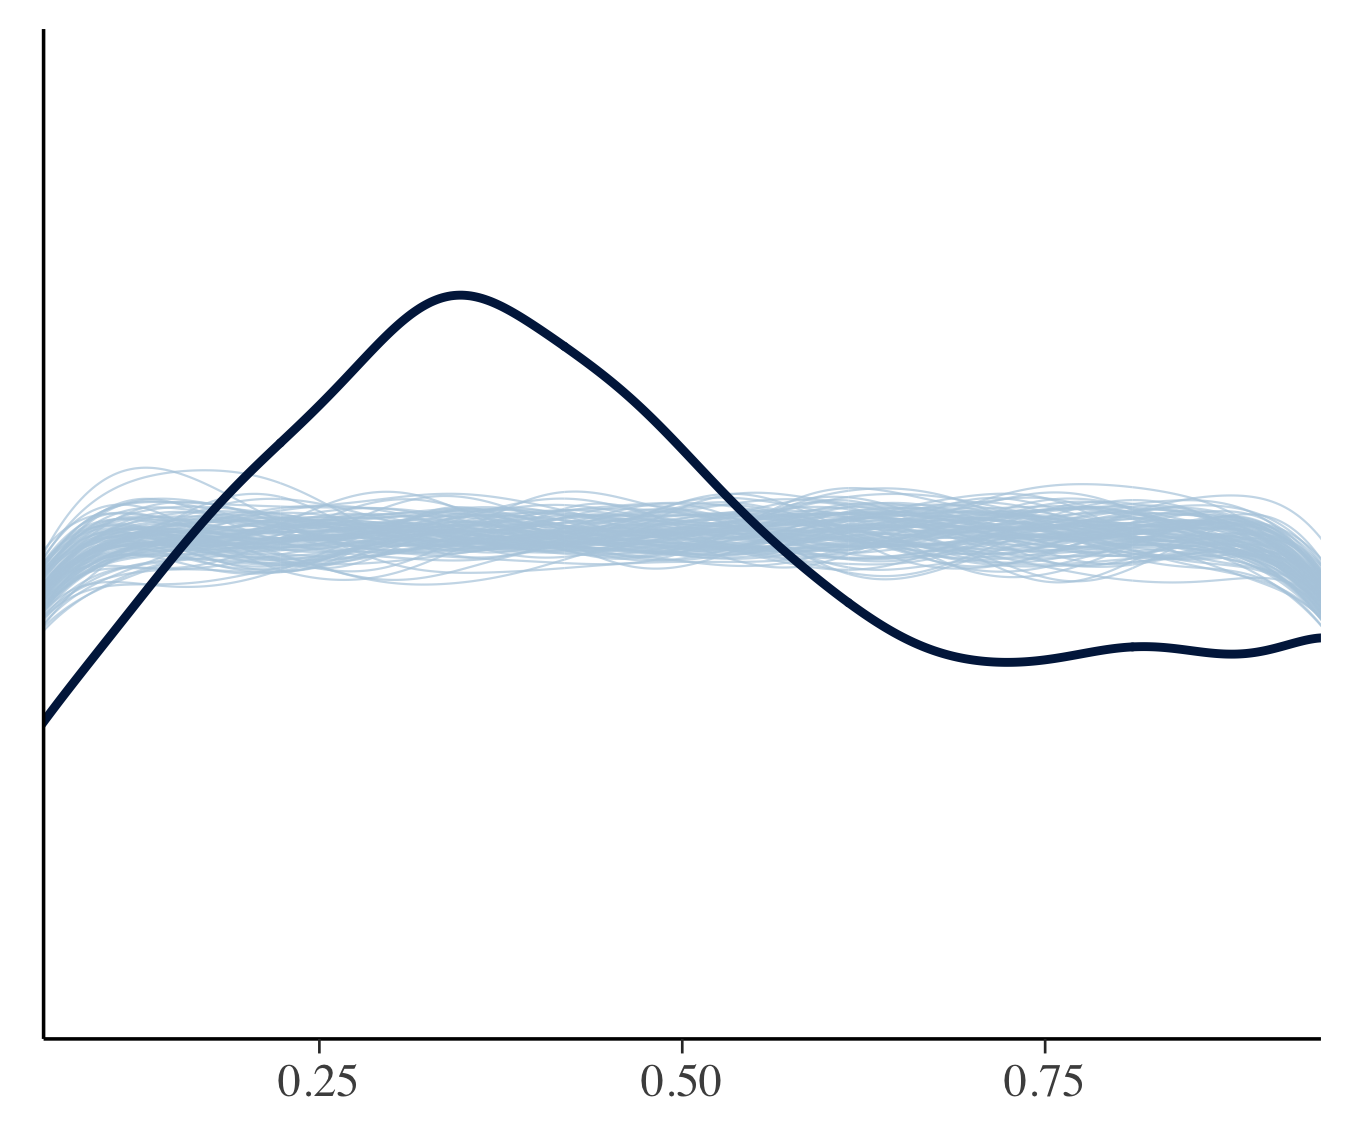
\includegraphics[width=\textwidth]{ppc_loo_pit_overlay1.png}
% % \caption{Model 1}
% % \end{subfigure}
% % ~
% % \begin{subfigure}{0.31\textwidth}
% % 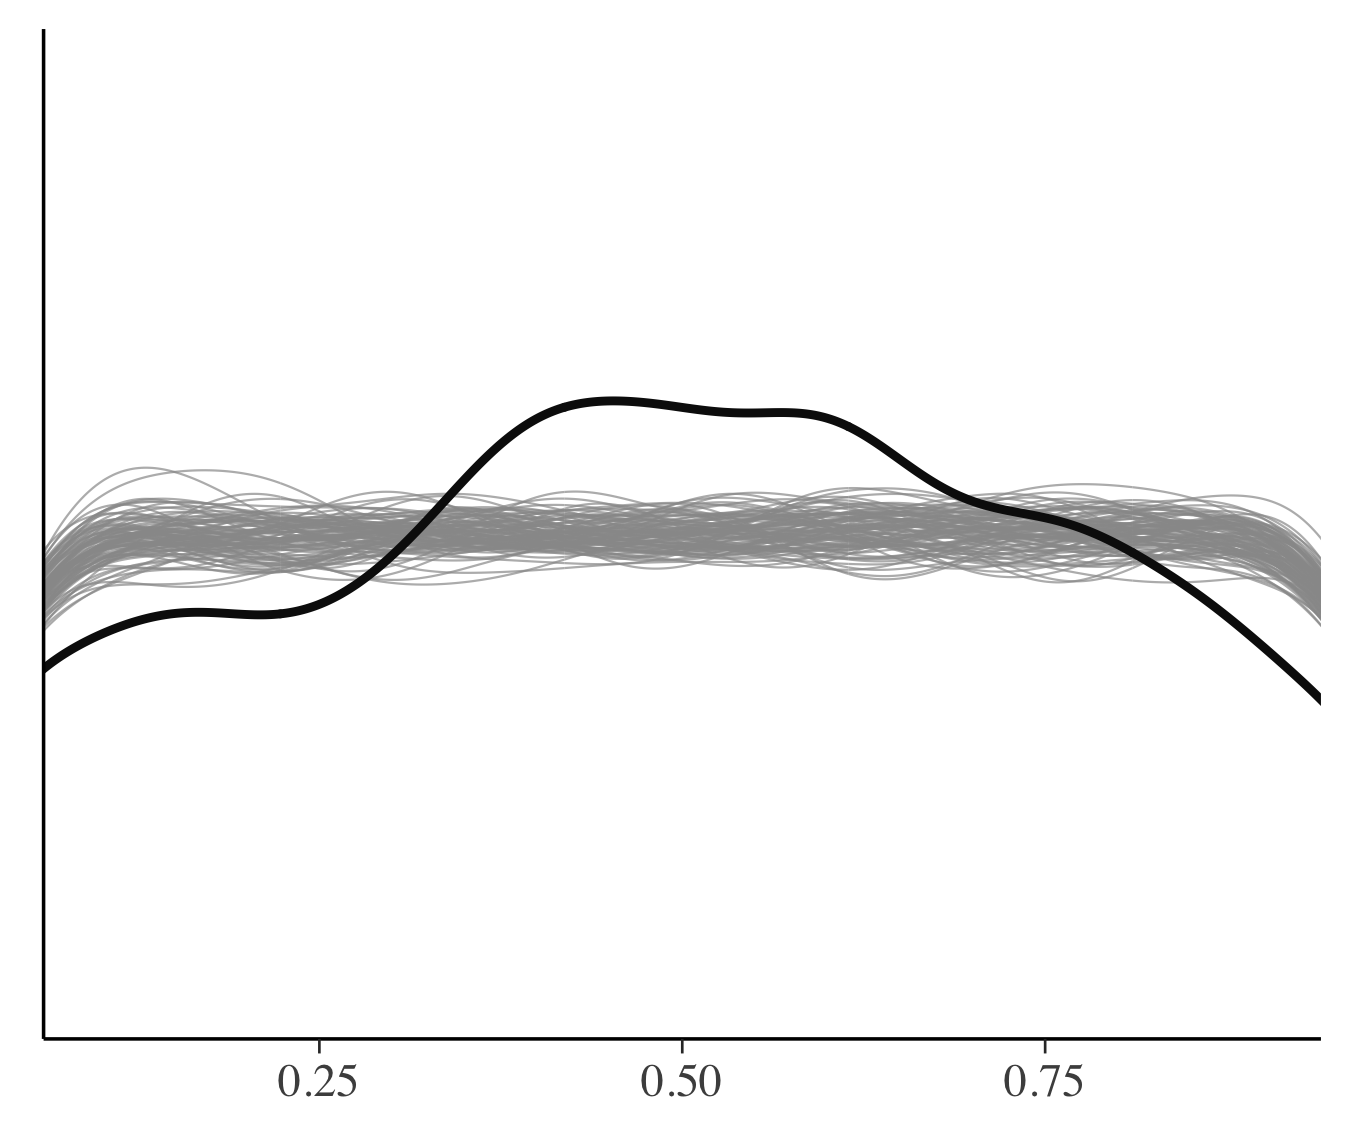
\includegraphics[width=\textwidth]{ppc_loo_pit_overlay2.png}
% % \caption{Model 2}
% % \end{subfigure}
% % ~
% % \begin{subfigure}{0.31\textwidth}
% % 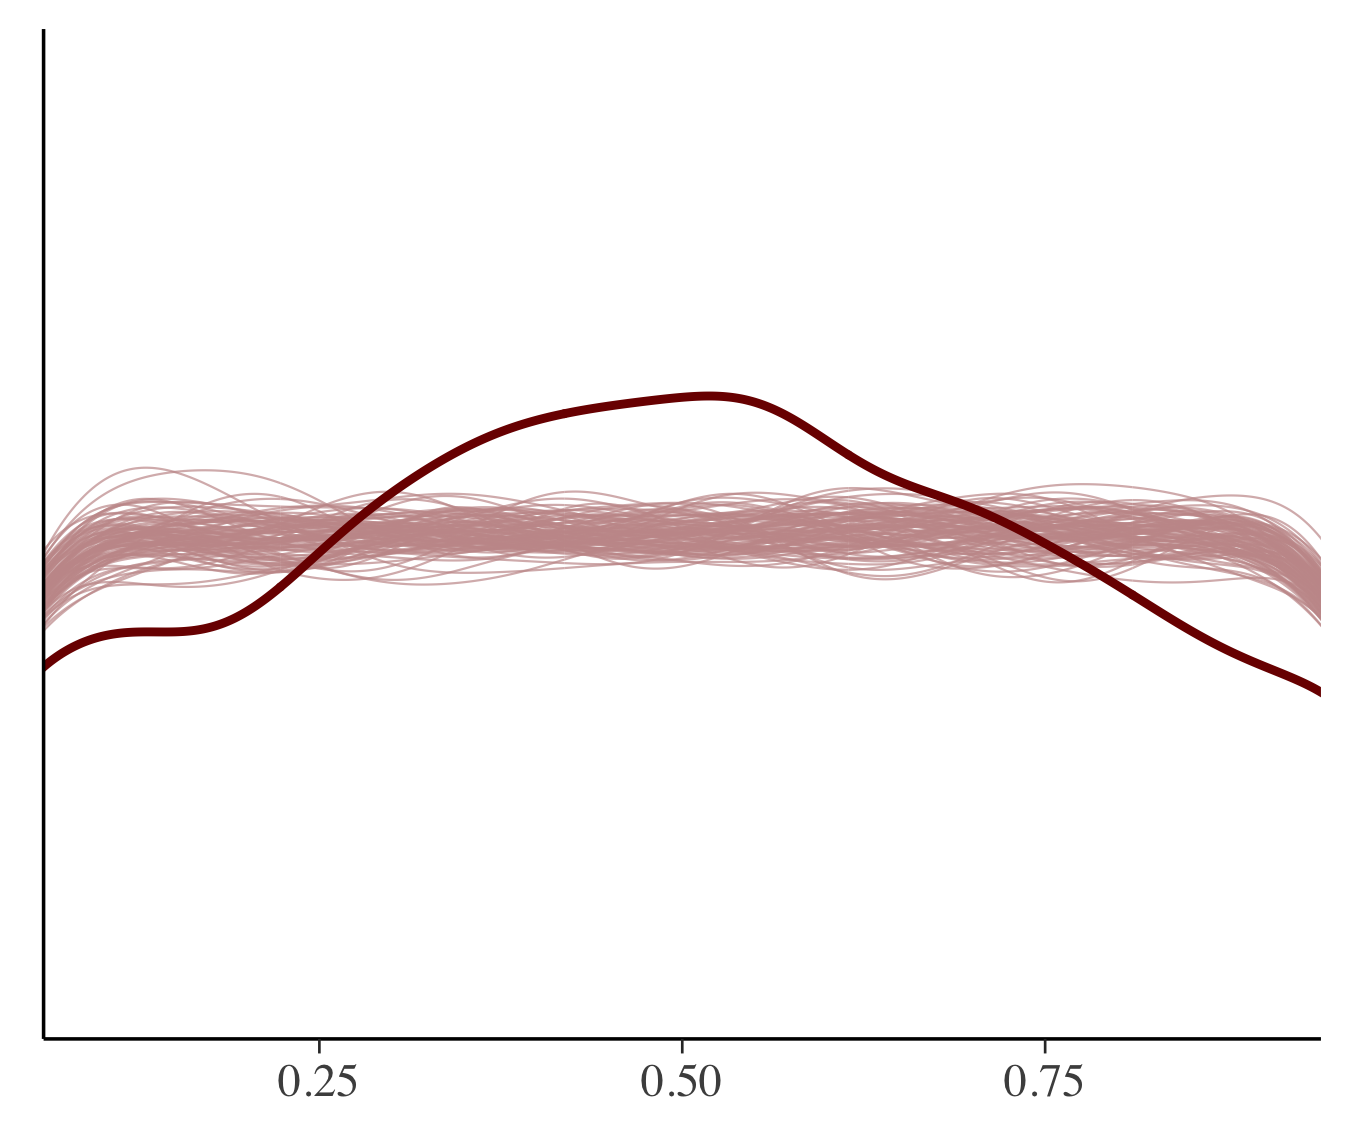
\includegraphics[width=\textwidth]{ppc_loo_pit_overlay3.png}
% % \caption{Model 3}
% % \end{subfigure}
% % \end{figure}

% % \vspace{2\baselineskip}
% % {\scriptsize EDIT 2020: These plots use boundary corrected KDE which is a better
% % choice than the non-boundary corrected KDE used in the plots in the
% % paper and the 2019 lecture.}

% \end{frame}

\begin{frame}{Brute-force LOO}

\begin{list1}
\item Re-run MCMC $n$ times to sample from $p(\theta \mid x_{-i},y_{-i})$
  \begin{itemize}
  \item can take a lot of time
  \item<2-> or high parallelization\\
    Cooper, Vehtari, Forbes, Kennedy, and Simpson (2023). Bayesian
    cross-validation by parallel Markov chain Monte
    Carlo. \textit{Statistics and Computing}, \textbf{34}:119. doi:10.1007/s11222-024-10404-w.
  \end{itemize}
\end{list1}

\end{frame}

\begin{frame}{Fast cross-validation}

\begin{list1}
\item Pareto smoothed importance sampling LOO (PSIS-LOO)
\item $K$-fold cross-validation
\end{list1}

\vspace{12\baselineskip}

{\small see \href{http://link.springer.com/article/10.1007/s11222-016-9696-4}{Vehtari, Gelman \& Gabry (2017a)} and \url{mc-stan.org/loo/}}

\end{frame}

\begin{frame}{Importance sampling leave-one-out cross-validation}

  \begin{list1}
  \item We want to compute ${\color{navyblue}p(y_i \mid x_i,x_{-i}, y_{-i})} = \int p(y_i \mid x_i,\theta){\color{blue} p(\theta \mid x_{-i}, y_{-i})} d\theta$
  \item<2-> Proposal distribution is full posterior $\theta^{(s)} \sim p(\theta \mid x,y)$
  \item<2-> Target distribution is LOO-posterior ${\color{blue} p(\theta \mid x_{-i}, y_{-i})}$
  \item<3-> Importance ratio
    \begin{align*}
    {\color{darkgreen} w_i^{(s)}} & = \frac{{\color{blue} p(\theta^{(s)} \mid x_{-i}, y_{-i})}}{p(\theta^{(s)} \mid x,y)}\propto \frac{1}{p(y_i \mid x_i,\theta^{(s)})}\\
      \uncover<4>{\color{darkgreen}\tilde{w}_i^{(s)}}&\uncover<4>{=\frac{{\color{darkgreen} w_i^{(s)}}}{\sum_{s'=1}^S {\color{darkgreen} w_i^{(s')}}}}
    \end{align*}
    % \begin{itemize}
    % \item self-normalized IS
    % \end{itemize}
  \end{list1}

  % \begin{itemize}
  % \item<4->Is the variance finite?
  %   \begin{itemize}
  %   \item no general analytic solution
  %   \end{itemize}
  % \end{itemize}
\end{frame}

\begin{frame}{}

  \only<1>{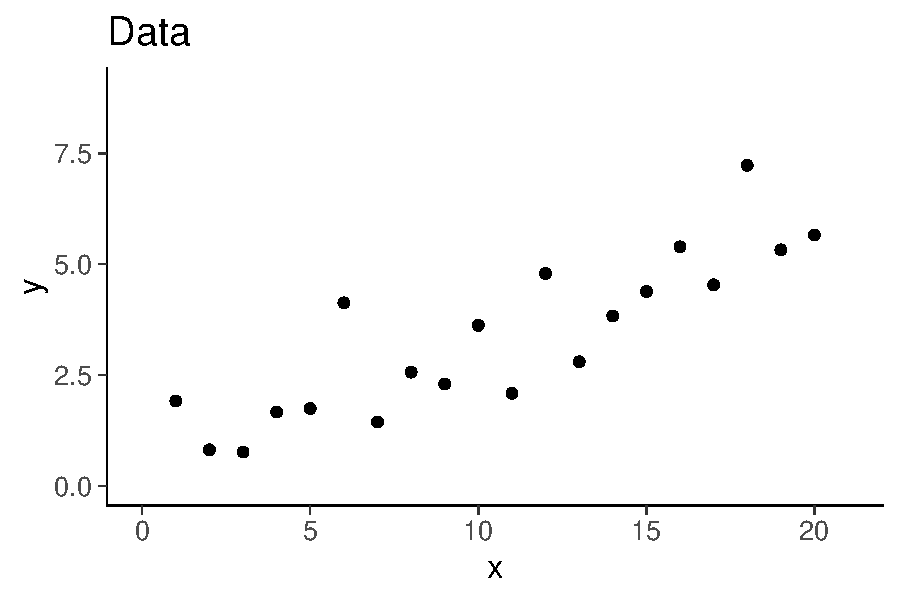
\includegraphics[width=10cm]{fakedata.pdf}}
  \only<2>{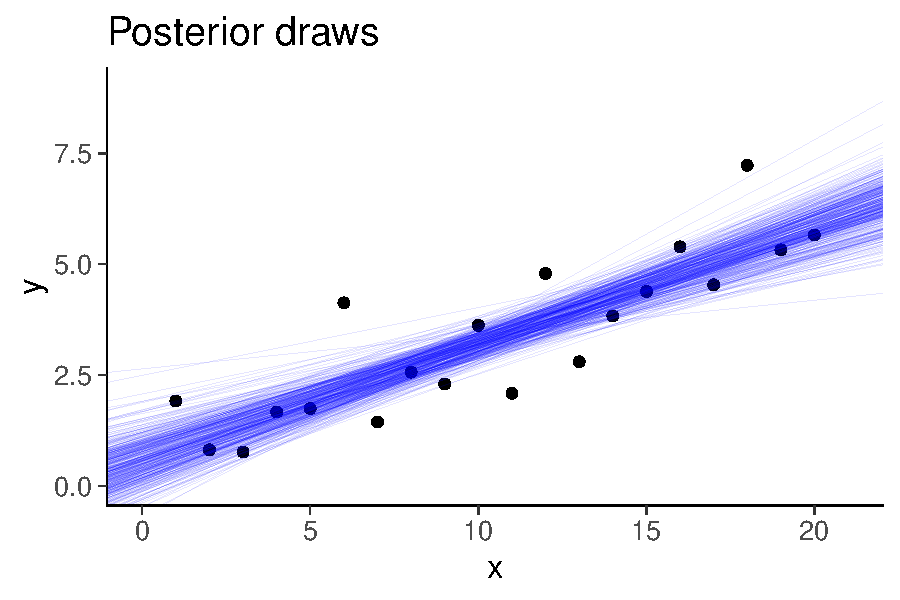
\includegraphics[width=10cm]{fakedraws.pdf}}
  \only<3>{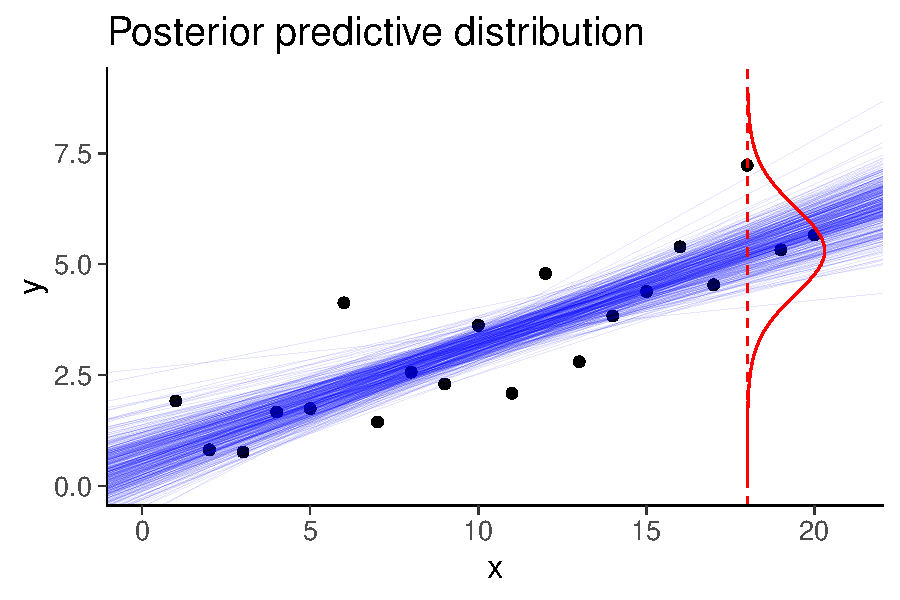
\includegraphics[width=10cm]{fakepostpred.pdf}}
  \only<4>{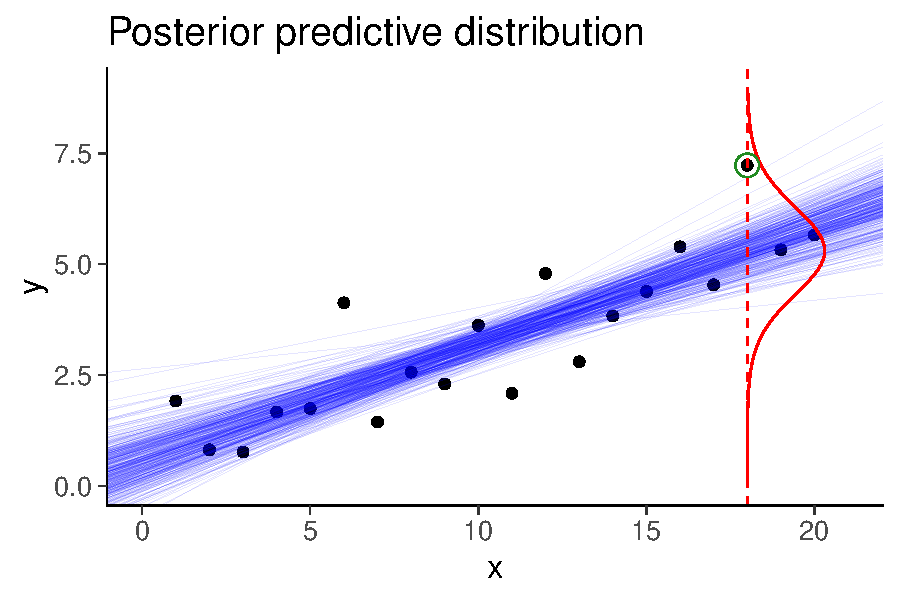
\includegraphics[width=10cm]{fakepostpred18.pdf}}
  \only<5>{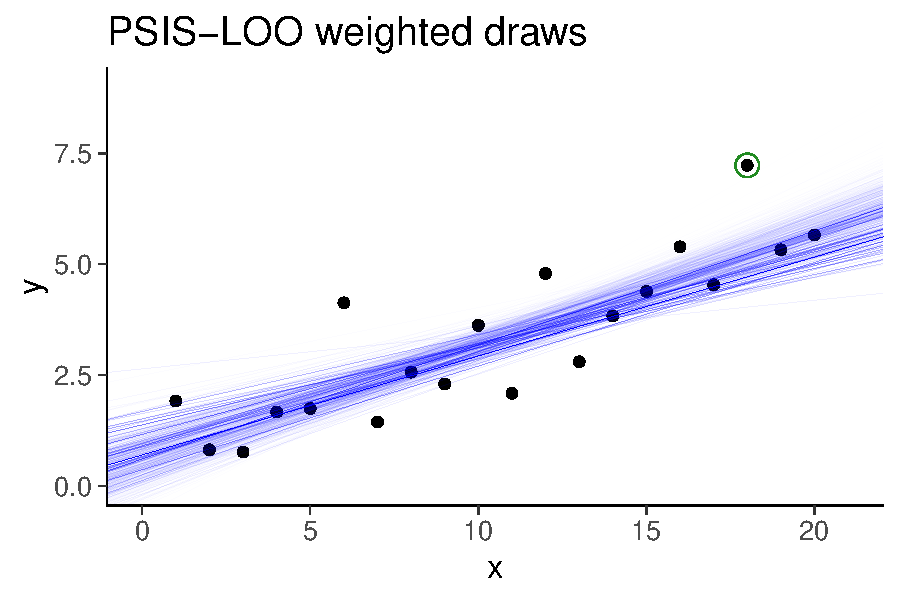
\includegraphics[width=10cm]{fakepsisdraws.pdf}}
  \only<6>{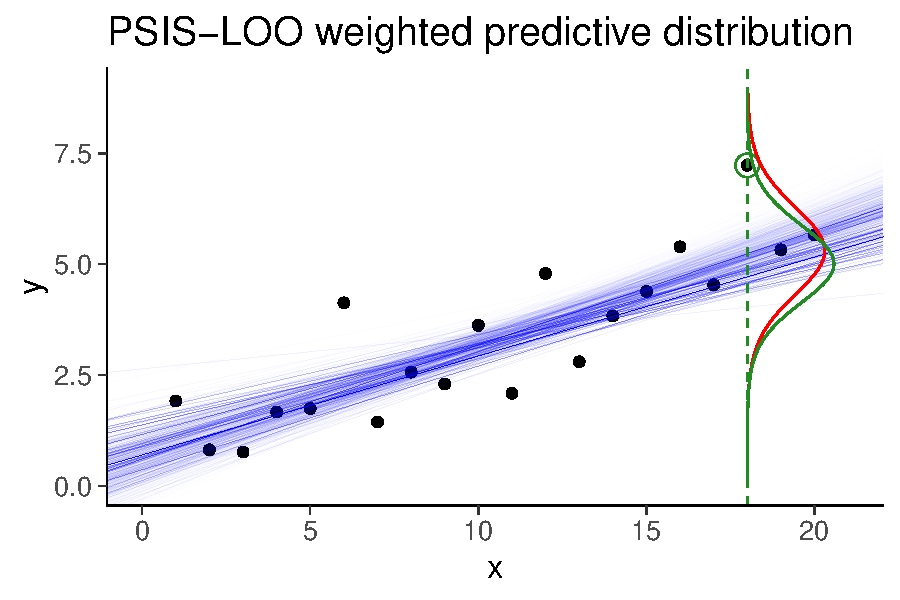
\includegraphics[width=10cm]{fakepsispostpred.pdf}}
  \\
  \only<2>{$\theta^{(s)} \sim p(\theta \mid x,y)$}
  \only<3-4>{$\theta^{(s)} \sim p(\theta \mid x,y), \quad p(\tilde{y} \mid \tilde{x},x,y) \approx \frac{1}{S}\sum_{s=1}^S p(\tilde{y} \mid \tilde{x},\theta^{(s)})$ }
  \only<5>{$\theta^{(s)} \sim p(\theta \mid x,y) , \quad {\color{darkgreen}  w_i^{(s)}} = p(\theta^{(s)} \mid x_{-i},y_{-i}) / p(\theta^{(s)} \mid x,y)$\\ \vspace{0.2\baselineskip} }
  \only<6->{$\theta^{(s)} \sim p(\theta \mid x,y), \quad \vspace{0.2\baselineskip}
    {\color{darkgreen}  w_i^{(s)}} = p(\theta^{(s)} \mid x_{-i},y_{-i}) / p(\theta^{(s)} \mid x,y) $\\ \vspace{0.2\baselineskip}
  $p(y_i \mid x_i,x_{-i},y_{-i}) \approx \sum_{s=1}^S [{\color{darkgreen}  \tilde{w}_i^{(s)}} p(y_i \mid x_i,\theta^{(s)})]$}%\only<6>{, where $w \leftarrow \mbox{PSIS}(r)$}
  % \only<6-8>{$\theta^{(s)} \sim p(\theta \mid x,y)$\\ \vspace{0.2\baselineskip} $ r_i^{(s)} = p(\theta^{(s)} \mid x_{-i},y_{-i}) / p(\theta^{(s)} \mid x,y) \propto 1/p(y_i \mid x_i,\theta^{(s)})$\\ \vspace{0.2\baselineskip} }
  % \only<7>{$\log(1/p(y_i \mid x_i,\theta^{(s)})) = -\mbox{log\_lik}[i]$}
  % \only<9-10>{$\theta^{(s)} \sim p(\theta \mid x,y)$\\ \vspace{0.2\baselineskip}
  %   $ r_i^{(s)} = p(\theta^{(s)} \mid x_{-i},y_{-i}) / p(\theta^{(s)} \mid x,y) \propto 1/p(y_i \mid x_i,\theta^{(s)})$\\ \vspace{0.2\baselineskip}
  % $p(y_i \mid x_i,x_{-i},y_{-i}) \approx \sum_{s=1}^S [w_i^{(s)} p(y_i \mid x_i,\theta^{(s)})]$}\only<10>{, where $w \leftarrow \mbox{PSIS}(r)$}
  
\end{frame}

\begin{frame}{Pareto smoothed importance sampling LOO}

  \vspace{-0.7\baselineskip}
  \begin{list1}
  \item ${\color{navyblue}p(y_i \mid x_i,x_{-i}, y_{-i})} = \int p(y_i \mid x_i,\theta){\color{blue} p(\theta \mid x_{-i}, y_{-i})} d\theta$
  \item Proposal $p(\theta \mid x,y)$ and target ${\color{blue} p(\theta \mid x_{-i}, y_{-i})}$
  \item Importance ratio
    \begin{align*}
    {\color{darkgreen} w_i^{(s)}} & = \frac{{\color{blue} p(\theta^{(s)} \mid x_{-i}, y_{-i})}}{p(\theta^{(s)} \mid x,y)}\propto \frac{1}{p(y_i \mid x_i,\theta^{(s)})}\\
      {\color{darkgreen}\tilde{w}_i^{(s)}}&{=\frac{{\color{darkgreen} w_i^{(s)}}}{\sum_{s'=1}^S {\color{darkgreen} w_i^{(s')}}}}\\
      p(y_i \mid x_i,x_{-i},y_{-i}) & \approx \sum_{s=1}^S \left[{\color{darkgreen}  \tilde{w}_i^{(s)}} p(y_i \mid x_i,\theta^{(s)})\right] \\
                                  & \uncover<2->{\approx  \frac {\sum_{s=1}^S \left[{\color{darkgreen}  {w}_i^{(s)}} p(y_i \mid x_i,\theta^{(s)})\right]}{\sum_{s'=1}^S {\color{darkgreen} w_i^{(s')}}}} \\
                                  & \uncover<3->{\approx \frac{1}{\frac{1}{S}\sum_{s'=1}^S {\color{darkgreen} w_i^{(s')}}} } \uncover<4->{ = \frac{1}{\frac{1}{S}\sum_{s=1}^S {\frac{1}{p(y_i \mid x_i,\theta^{(s)})}}} }
    \end{align*}
  \end{list1}

  \begin{list1}
  \item The variability of importance weights matter
    \begin{list2}
    \item Pareto-$\hat{k}$ diagnostic
    \item Pareto smoothed importance sampling LOO (PSIS-LOO)
    \end{list2}
  \end{list1}
\end{frame}

\begin{frame}{Pareto smoothed importance sampling LOO}

  \begin{list1}
  \item ${\color{navyblue}p(y_i \mid x_i,x_{-i}, y_{-i})} = \int p(y_i \mid x_i,\theta){\color{blue} p(\theta \mid x_{-i}, y_{-i})} d\theta$\\
    \begin{align*}
      p(y_i \mid x_i,x_{-i},y_{-i}) & \approx \sum_{s=1}^S \left[{\color{darkgreen}  \tilde{w}_i^{(s)}} p(y_i \mid x_i,\theta^{(s)})\right] \\
                                  & {\approx \frac{1}{\frac{1}{S}\sum_{s'=1}^S {\color{darkgreen} w_i^{(s')}}} }
    \end{align*}
  \end{list1}

  \begin{list1}
  \item The variability of importance weights matter
    \begin{list2}
    \item Pareto-$k$ diagnostic
    \item Pareto smoothed importance sampling LOO (PSIS-LOO)
    \end{list2}
  \end{list1}
\end{frame}

\begin{frame}{}
%XXX fiix figures
  \only<1>{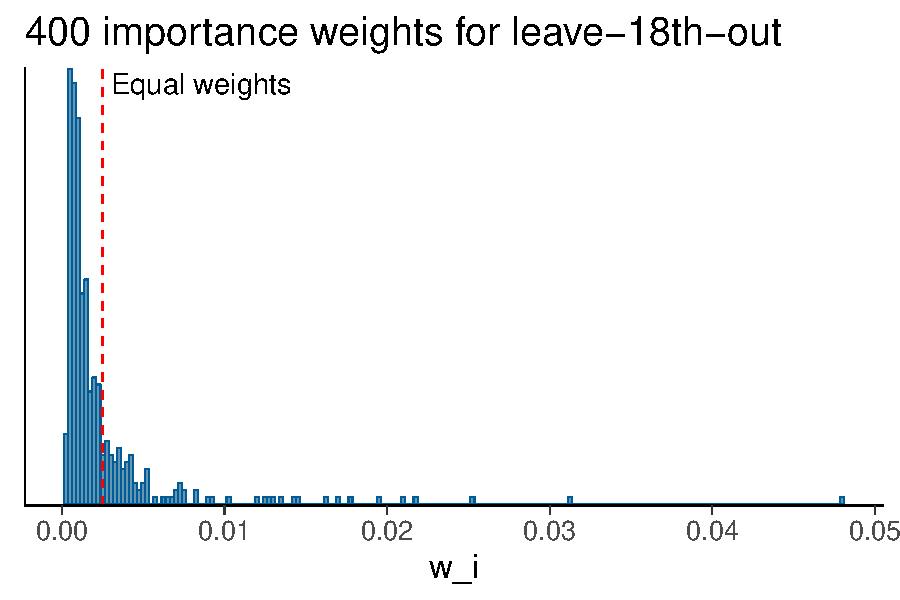
\includegraphics[width=10cm]{fakepsisweights.pdf}}
  \only<2->{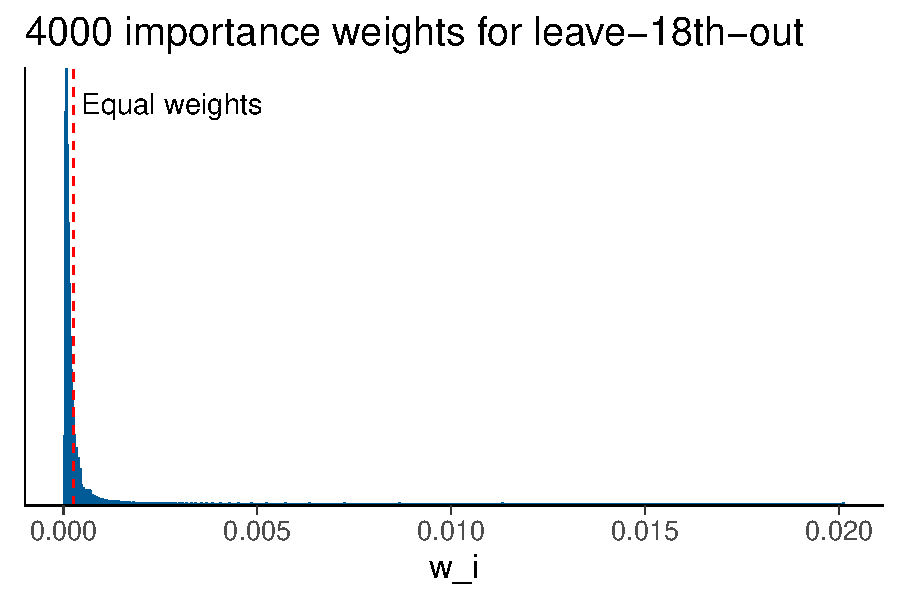
\includegraphics[width=10cm]{fakepsisweights4000.pdf}}
  \\
  \onslide<3->{ESS $\approx 1/ {\sum_{s=1}^S ({\color{darkgreen}\tilde{w}^{(s)}})^2} \approx$ 459\\  \vspace{0.2\baselineskip}}
  \onslide<4>{Pareto $\hat{k}$ $\approx$ 0.52
  \vspace{-\parskip}
    \begin{list2}
    \item Pareto $\hat{k}$ estimates the tail shape which determines the convergence rate of PSIS. Less than 0.7 is ok.}
\end{list2}
  \onslide<3->{\vfill\small see \href{https://jmlr.org/papers/v25/19-556.html}{Vehtari et al. (2024)}}
\end{frame}

\begin{frame}{Pareto-$\hat{k}$ diagnostic}

%  \begin{itemize}
   Pickands (1975): many distributions have tail ($x > u$) that
    is well approximated with Generalized Pareto distribution (GPD)
%  \end{itemize}

    {
      \vspace{-0.5\baselineskip}
\only<1>{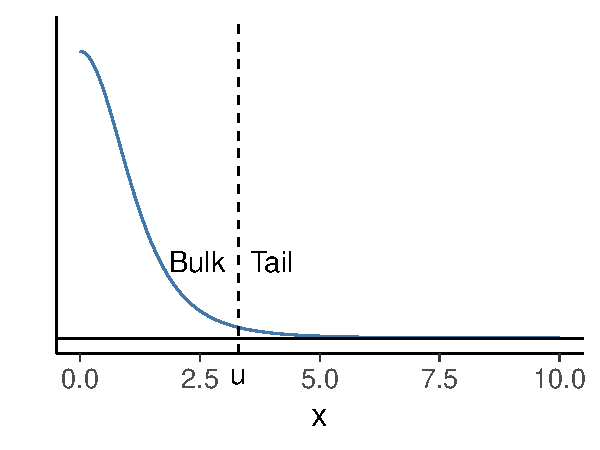
\includegraphics[width=9.5cm]{bulktail.pdf}}\only<2>{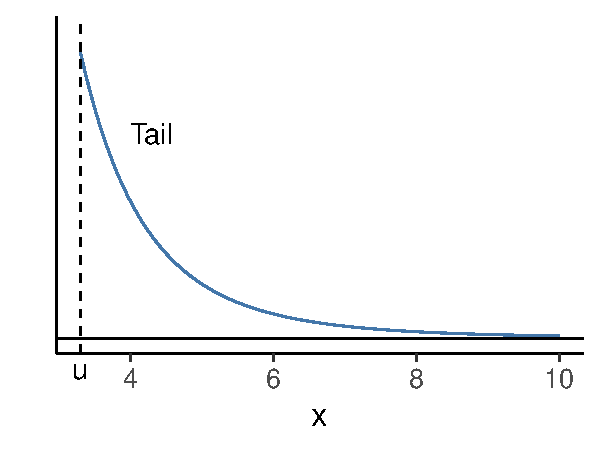
\includegraphics[width=9.5cm]{tail1.pdf}}\only<3>{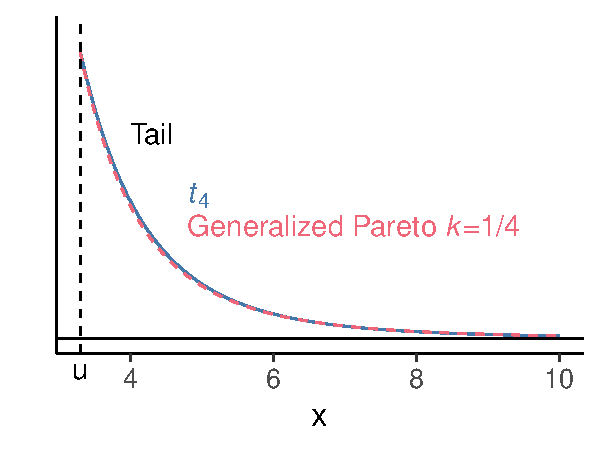
\includegraphics[width=9.5cm]{tail2.pdf}}\only<4>{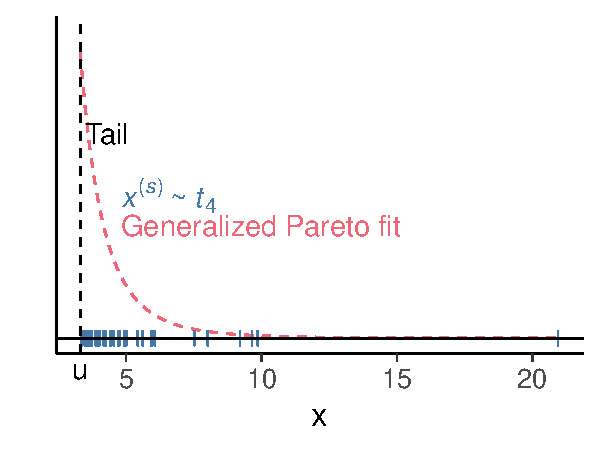
\includegraphics[width=9.5cm]{tail3.pdf}}
}

\end{frame}

\begin{frame}[fragile]

  \begin{itemize}
  \item Pareto-$\hat{k}$ for each leave-one-out fold indicates
    reliability of the PSIS-LOO approximation
  % \item High Pareto-$\hat{k}$ may also indicate model
  %   mis-specification, but can occur also in case of perfectly
  %   specified model
  \end{itemize}
  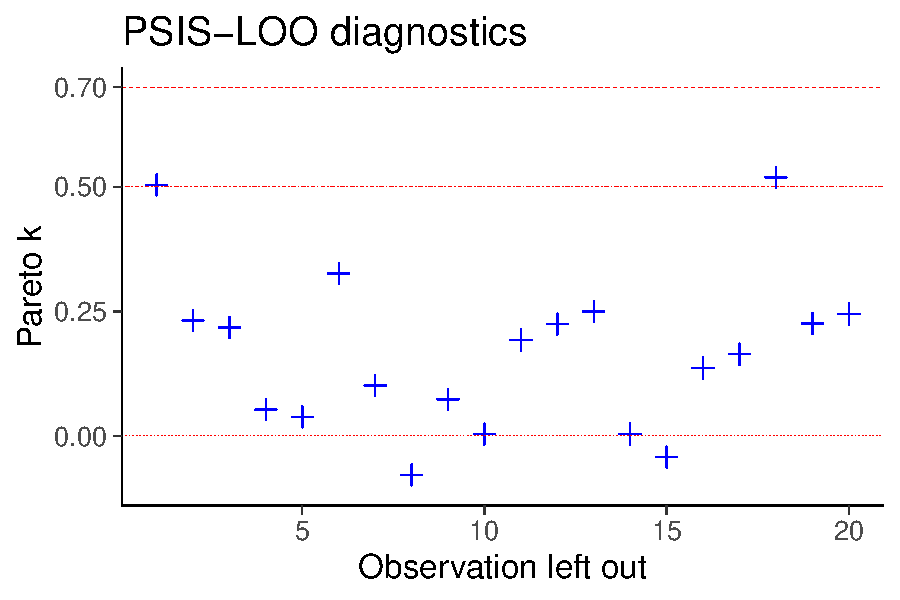
\includegraphics[width=10cm]{fakepks.pdf}

\end{frame}

\begin{frame}[fragile]

  \only<1>{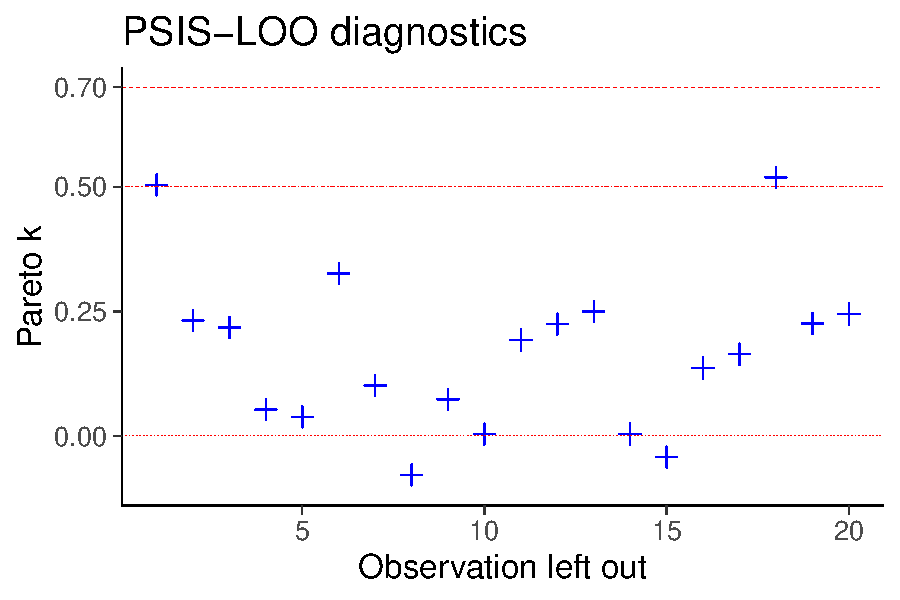
\includegraphics[width=10cm]{fakepks.pdf}}
  \only<2>{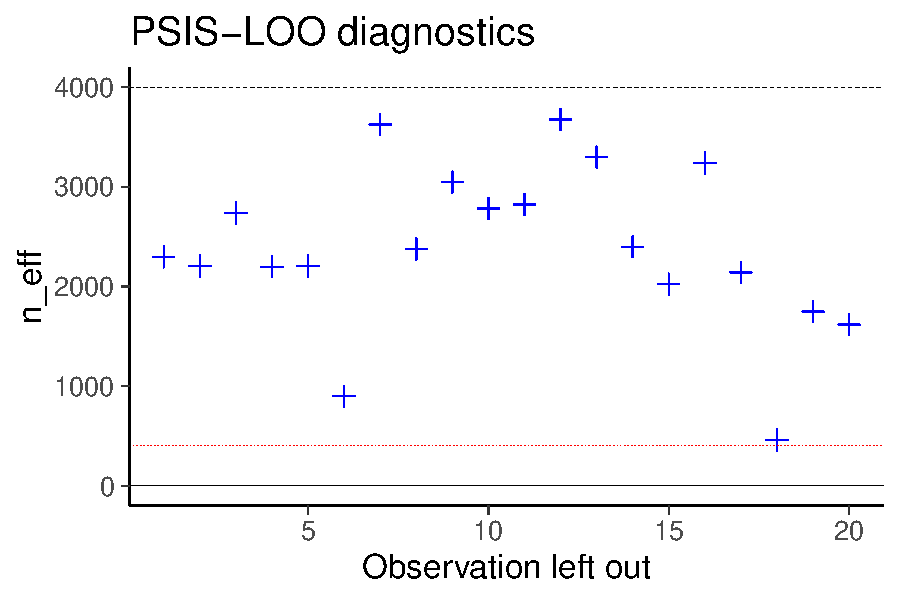
\includegraphics[width=10cm]{fakeneffs.pdf}}
  \\
\begin{minted}[fontsize=\scriptsize]{text}
All Pareto k estimates are good (k < 0.7).
\end{minted}

\end{frame}

\begin{frame}[fragile]
  \frametitle{{\tt loo} package}

\begin{minted}[gray,fontsize=\scriptsize]{text}
 Computed from 4000 by 20 log-likelihood matrix

         Estimate  SE
elpd_loo    -29.5 3.3
p_loo         2.7 1.0
\end{minted}
\begin{minted}[fontsize=\scriptsize]{text}
------
MCSE of elpd_loo is 0.1.
MCSE and ESS estimates assume MCMC draws (r_eff in [0.6, 1.2]).

All Pareto k estimates are good (k < 0.7).
See help('pareto-k-diagnostic') for details.
\end{minted}

{\vfill\small see more by \href{https://jmlr.org/papers/v25/19-556.html}{Vehtari et al. (2024)}}

\end{frame}

\begin{frame}[fragile]{Student retention -- loo computation}

\begin{minted}[fontsize=\footnotesize,escapeinside=||]{text}
> fit4 <- add_criterion(fit4, 'loo')
Pareto k diagnostic values:
                         Count Pct.    Min. ESS
|{\color{forestgreen}(-Inf, 0.7]   (good)     32    80.0%   114     }|
|{\color{red}   (0.7, 1]   (bad)       7    17.5%   <NA>    }|
|{\color{red}   (1, Inf)   (very bad)  1     2.5%   <NA>    }|
\end{minted}
\end{frame}

% \begin{frame}
%   \frametitle{Importance sampling}

%   \begin{itemize}
%   \item Having samples $\theta^s$ from $p(\theta^s \mid D)$
%     \begin{align*}
%       p(\tilde{y}_i \mid x_i,D_{-i})\approx\frac{\sum_{s=1}^Sp(\tilde{y}_i \mid \theta^s)w_i^s}{\sum_{s=1}^S w_i^s},
%     \end{align*}
%     where $w_i^s$ are importance weights and
%     \begin{align*}
%       w_i^s=\frac{p(\theta^s \mid x_i,D_{-i})}{p(\theta^s \mid D)}\propto\frac{1}{\color{red} p(y_i \mid \theta^s)}.
%     \end{align*}
% % \pause
% %   \item If evaluated with $\tilde{y}_i=y_i$ 
% %     \begin{align*}
% %       p(y_i \mid x_i,D_{-i})\approx\frac{1}{\sum_{s=1}^S\frac{1}{p(y_i \mid \theta^s)}},
% %     \end{align*}
%   \end{itemize}

% \end{frame}

\begin{frame}{Pareto smoothed importance sampling (PSIS)}

  \vspace{-.5\baselineskip}
  
  \begin{list1}
    \item Replace the largest weights with ordered statistics of the
      fitted Pareto distribution
      \begin{list2}
      \item equivalent to using model to filter the noise out of the weights
      \end{list2}
    \item<2-> Works well if $\hat{k}<0.7$
      \item<2-> Reduced variability compared to the plain IS
      \item<2-> Reduced bias compared to the truncated IS
      \item<3-> Asymptotically consistent under some mild conditions
      \end{list1}
      \vspace{7\baselineskip}

      
    {\vfill\small see more by \href{https://jmlr.org/papers/v25/19-556.html}{Vehtari et al. (2024)}}
\end{frame}

\begin{frame}{Pareto-$\hat{k}$ and convergence rate of PSIS}

  \begin{itemize}
  \item CLT says that to half the MCSE, need 4 times bigger S
  \item<2-> If Pareto-$\hat{k} \approx 0.7$, to half the MCSE, need 10 times bigger S
  \item<3-> If Pareto-$\hat{k}>1$, to half the MCSE, nothing helps
  \end{itemize}
  
\end{frame}

\begin{frame}[fragile]
  \frametitle{Stan code }

  \vspace{\baselineskip}
  $ \log(w_i^{(s)}) = \log(1/p(y_i \mid x_i,\theta^{(s)})) = $ \rinline/log_lik[i]/
  \vspace{\baselineskip}

  \pause
\begin{minted}[fontsize=\footnotesize,highlightlines={4,9}]{stan}
model {
  alpha ~ normal(pmualpha, psalpha);
  beta ~ normal(pmubeta, psbeta);
  y ~ normal(mu, sigma);
}
generated quantities {
  vector[N] log_lik;
  for (i in 1:N)
    log_lik[i] = normal_lpdf(y[i] | mu[i], sigma);
}
\end{minted}

  \begin{list1}
  \item<3-> RStanARM and brms compute \rinline/log_lik/ by default
  \end{list1}
  
\end{frame}

\begin{frame}[fragile]
  \frametitle{loo()}

  \begin{list1}
  \item<+-> RStan (\rinline/log_lik/ in gen. quantities)\\
    \rinline/loo(fit)/
  \item<+-> CmdStanR (\rinline/log_lik/ in gen. quantities)\\
    \rinline/fit$loo()/ %$
  \item<+-> RStanARM, brms\\
    \rinline/loo(fit)/
  \item<+-> brms alternative\\
    \rinline/fit <- add_criterion(fit, "loo")/
  \end{list1}
  
\end{frame}

\begin{frame}{High Pareto-$\hat{k}$ values}

\begin{list1}
\item<+-> High Pareto-$\hat{k}$ value indicates the target distribution
  (LOO posterior) is very different from the proposal distribution
  (full data posterior)
\item<+-> This can be caused by
  \begin{itemize}
  \item well specified, but very flexible model
    \begin{itemize}
    \item e.g. hierarchical model with one parameter per observation
    \item indicated by large \rinline/p/ and \rinline/p_loo/ (e.g. $N/5 < $ \rinline/p,p_loo/ $<$ \rinline/p/)
    \item moment matching or integrated LOO may help
    \end{itemize}
  \item<+-> misspecified model / outliers
    \begin{itemize}
    \item indicated by \rinline/p_loo/ $\ll$ \rinline/p/, or \rinline/p_loo/ $>$ \rinline/p/
    \item improve model, check data
    \end{itemize}
  \end{itemize}
\item<+-> See more in \href{https://users.aalto.fi/~ave/modelselection/CV-FAQ.html}{CV-FAQ}

\end{list1}

\end{frame}

\begin{frame}[fragile]
  \frametitle{What if many high Pareto-$\hat{k}$'s}

  \begin{list1}
  \item<+-> \rinline/rstan::loo(..., moment_match = TRUE)/\\
    \rinline/brms::loo(..., moment_match = TRUE)/\\
    support implicitly adaptive importance sampling with moment
    matching algorithm by
    \href{https://doi.org/10.1007/s11222-020-09982-2}{Paananen et al. (2021)}.  See \url{http://mc-stan.org/loo/articles/loo2-moment-matching.html}
  \item<+-> \rinline/rstanarm::loo(..., k_threshold = 0.7)/\\
    \rinline/brms::loo(..., k_threshold = 0.7)/\\
    runs MCMC for the folds with $\hat{k}$ above the threshold
  \item<+-> Integrated LOO (for some models)\\
    See \url{https://users.aalto.fi/~ave/modelselection/roaches.html}
  \item<+-> Use $K$-fold-CV (more about this later)\\
    \rinline/rstanarm::kfold(..., K=10)/\\
    \rinline/brms::kfold(..., K=10)/\\
    RStan/CmdStanR vignette \url{http://mc-stan.org/loo/articles/loo2-elpd.html}
  \end{list1}
  
\end{frame}

\begin{frame}[fragile]{Student retention -- loo computation}

PSIS-LOO

\begin{minted}[fontsize=\footnotesize,escapeinside=||]{text}
> fit4 <- add_criterion(fit4, 'loo')
Pareto k diagnostic values:
                         Count Pct.    Min. ESS
|{\color{forestgreen}(-Inf, 0.7]   (good)     32    80.0%   114     }|
|{\color{red}   (0.7, 1]   (bad)       7    17.5%   <NA>    }|
|{\color{red}   (1, Inf)   (very bad)  1     2.5%   <NA>    }|
\end{minted}

\pause
PSIS-LOO + moment matching + reloo
\begin{minted}[fontsize=\footnotesize,escapeinside=||]{text}
> ...(fit4, 'loo', |\highlight{moment_match=TRUE, reloo=TRUE, overwrite=TRUE}|)
|{\color{forestgreen}All Pareto k estimates are good (k < 0.7).}|
\end{minted}

  \vfill
{\color{gray}\footnotesize\href{https://doi.org/10.1007/s11222-020-09982-2}{Paananen, Piironen, Bürkner, and Vehtari (2021). Implicitly adaptive importance sampling. \textit{Statistics and Computing}, 31, 16.}}
  
\end{frame}

\begin{frame}{Cross-validation for model assessment}

\begin{list1}
\item CV is good for model assessment when application specific utility/cost functions are used
  \begin{list2}
  \item e.g. in concrete quality prediction reported that the absolute
    error is smaller than X with 90\% probability
  \end{list2}
\item<2-> Also useful in model checking in similar way as posterior
  predictive checking (PPC)
  \begin{list2}
  \item checking calibration of leave-one-out predictive posteriors
    (\rinline/ppc_loo_pit/ in \rinline/bayesplot/)
  \item model misspecification diagnostics\\ (e.g. Pareto-$k$ and \rinline/p_loo/)
  \end{list2}
  {\small see demos \url{https://users.aalto.fi/~ave/casestudies.html}}
\end{list1}

\end{frame}


% \begin{frame}{Radon example}

%    PSIS-LOO diagnostics
%    \includegraphics[width=.8\textwidth]{radon1k.pdf}

% {\small see \href{http://link.springer.com/article/10.1007/s11222-016-9696-4}{Vehtari, Gelman \& Gabry (2017a)}}
   
%  \end{frame}


\begin{frame}{Sometimes cross-validation is not needed}

\vspace{-0.5\baselineskip}

  \begin{list1}
  \item Posterior predictive checking is often sufficient\\
    \vspace{0.5\baselineskip}
    \includegraphics[width=11cm]{mesquite_ppc.pdf}\\
  \vspace{-0.1\baselineskip} {Predicting the yields of mesquite bushes.\\
    \color{gray} \footnotesize
    Gelman, Hill \& Vehtari (2020): Regression and Other Stories, Chapter 11.}\\
  \vspace{-0.8\baselineskip}
\end{list1}
{\footnotesize
  \begin{list2}
  \item<2-> BDA3, Chapter 6
  \vspace{-0.6\parskip}
  \item<2-> Gabry, Simpson, Vehtari, Betancourt, Gelman
    (2019). Visualization in Bayesian workflow. JRSS A, \url{https://doi.org/10.1111/rssa.12378}
  \vspace{-0.6\parskip}
  \item<2-> \url{mc-stan.org/bayesplot/articles/graphical-ppcs.html}
   \end{list2}}
\end{frame}



% \begin{frame}[fragile]{Student retention -- loo computation}

% PSIS-LOO

% \begin{minted}[fontsize=\footnotesize,escapeinside=||]{text}
% > fit6 <- add_criterion(fit6, 'loo')
% Pareto k diagnostic values:
%                          Count Pct.    Min. n_eff
% (-Inf, 0.5]   (good)     34    85.0%   558       
%  (0.5, 0.7]   (ok)        5    12.5%   226       
%    (0.7, 1]   (bad)       1     2.5%   215       
%    (1, Inf)   (very bad)  0     0.0%   <NA>
% \end{minted}

% PSIS-LOO + moment matching  
% \begin{minted}[fontsize=\footnotesize,escapeinside=||]{text}
% > ...(fit6, 'loo', moment_match=TRUE, overwrite=TRUE)
% All Pareto k estimates are good (k < 0.7).
% \end{minted}
  
%   \vspace{0.5\baselineskip}
% {\color{gray}\footnotesize\href{https://doi.org/10.1007/s11222-020-09982-2}{Paananen, Piironen, Bürkner, and Vehtari (2021). Implicitly adaptive importance sampling. \textit{Statistics and Computing}, 31, 16.}}
% \end{frame}

\begin{frame}
  \frametitle{Next week}

  \begin{itemize}
  \item Model comparison with LOO-CV
  \item When is cross-validation applicable?
    \begin{list2}
    \item data generating mechanisms and prediction tasks
    \item leave-many-out cross-validation
    \end{list2}
  \item $K$-fold cross-validation
  \item {\footnotesize Related methods (WAIC, *IC, BF)}
  \item Model averaging
  \item Hypothesis testing
  \item Potential overfitting in model selection
  % \item<2-> Part 2: Projective Inference in High-dimensional Problems:
  %   Prediction and Feature Selection
  \end{itemize}
  
\end{frame}

\end{document}

% \begin{frame}{Sometimes cross-validation is not needed}

%   \begin{list1}
%   \item With good priors that keep the prior on predictive space
%     consistent, no need to do model selection to avoid
%     overfitting
%   \end{list1}
%   \vspace{-0.6\baselineskip}
%   \only<1>{\includegraphics[width=8cm]{overfit_simdata.pdf}}
%   \only<2>{\includegraphics[width=8cm]{overfit_elpd_poly.pdf}\\
%   Polynomial with wide priors implies prior favoring overfitting}
%    \only<3>{\includegraphics[width=8cm]{overfit_elpd_GP.pdf}\\
%  GP basis functions imply prior not favoring overfitting}
  
% \end{frame}

% \begin{frame}{}

% {\Large\color{navyblue} Model comparison}

% \begin{list1}
% \item ``A popular hypothesis has it that primates with larger brains
%   produce more energetic milk, so that brains can grow quickly'' (from
%   Statistical Rethinking)
%   \begin{list2}
%     \item Model 1: formula = kcal.per.g $\sim$ neocortex
%     \item Model 2: formula = kcal.per.g $\sim$ neocortex + log(mass)
%   \end{list2}
% \end{list1}

% \vspace{10\baselineskip}
% {\small \url{mc-stan.org/loo/articles/loo2-example.html}}

% \end{frame}

% \begin{frame}

%   \only<1-2>{\includegraphics[width=10cm]{milkelpdloo.pdf}}
%   \only<3>{\includegraphics[width=10cm]{milkelpdloo2.pdf}}
%   \\
%   \only<2-3>{Model 1 elpd\_loo $\approx$ 3.7, SE=1.8\\
%   Model 2 elpd\_loo $\approx$ 8.4, SE=2.8}

% \end{frame}

% \begin{frame}[fragile]

%   {\includegraphics[width=10cm]{milkelpddiff.pdf}}
%   \\
%   {\scriptsize
% \begin{lstlisting}
% Model comparison: 
% (negative 'elpd_diff' favors 1st model, positive favors 2nd) 

% elpd_diff        se 
%       4.7       2.7 
% \end{lstlisting}}

% \end{frame}

% \begin{frame}

%   {\Large\color{navyblue} Arsenic well example -- Model comparison}

   
%    \includegraphics[width=.8\textwidth]{arsenic12d.pdf}

%    An estimated difference in ${\rm elpd}_{\rm loo}$ of 16.4 with SE of 4.4.
   
% {\small see \href{http://link.springer.com/article/10.1007/s11222-016-9696-4}{Vehtari, Gelman \& Gabry (2017a)}}
% \end{frame}

\begin{frame}{Arsenic well example -- Model comparison}

\begin{list1}
\item Logistic regression for predicting probability of switching well
  with high arsenic level in rural
  Bangladesh\\\vspace{0.25\baselineskip}
  \begin{list2}
    \item \color{set12}Model 1:\\ {\color{navyblue}log(arsenic) + distance}\\\vspace{0.25\baselineskip}
    \item \color{set13}Model 2:\\ {\color{navyblue}log(arsenic) + distance + education level}
  \end{list2}
\end{list1}

\vspace{10\baselineskip}
{\footnotesize Gelman, Hill \& Vehtari (2020): Regression and Other Stories, Chapter 13.}

\end{frame}

\begin{frame}{Arsenic well example -- Model comparison}
  
  {\includegraphics[height=6.5cm]{arsenicelpdloo.pdf}}
  % \only<3>{\includegraphics[width=10cm]{milkelpdloo2.pdf}}
  \\
  {{\color{set12}Model 1}: $\elpdHat{{\color{set12}\Ma}}{\yobs}\approx$ -1952, SE=16\\
    {\color{set13}Model 2}: $\elpdHat{{\color{set13}\Mb}}{\yobs}\approx$ -1938, SE=17}

\end{frame}

\begin{frame}[fragile]

  \frametitle{Arsenic well example -- Model comparison}

  \uncover<1-3>{\includegraphics[height=6.5cm]{arsenicelpddiff.pdf}}
  \only<2>{\includegraphics[height=6.5cm]{arsenicelpddiff_dens1.pdf}}
  \hspace{-1.1mm}\only<3>{\includegraphics[height=6.5cm]{arsenicelpddiff_dens2.pdf}}
  \hspace{-6.7cm}\only<4>{\includegraphics[height=6.5cm]{arsenicelpddiff_dens3.pdf}}
  \\
  Difference: $\elpdHat{{\color{set12}\Ma},{\color{set13}\Mb}}{\yobs}\approx$ -14.4, SE = 6.1
%   {\scriptsize
% \begin{lstlisting}
% > loo_compare(model1, model2)
%        elpd_diff se_diff
% model2   0.0       0.0  
% model1 -14.4       6.1  
% \end{lstlisting}}
% \vspace{-\baselineskip}
%     {\scriptsize \hspace{6cm} see \href{http://link.springer.com/article/10.1007/s11222-016-9696-4}{Vehtari, Gelman \& Gabry (2017a)}}
    
\end{frame}

\begin{frame}[fragile]
  \frametitle{Arsenic well example -- Model comparison}

  {\includegraphics[height=6.5cm]{arsenicelpddiff_dens3.pdf}}
  \\
\begin{minted}[fontsize=\scriptsize]{text}
> loo_compare(model1, model2)
       elpd_diff se_diff
model2   0.0       0.0  
model1 -14.4       6.1  
\end{minted}
\vspace{-\baselineskip}
    {\scriptsize \hspace{6cm} see \href{http://link.springer.com/article/10.1007/s11222-016-9696-4}{Vehtari, Gelman \& Gabry (2017a)}}
    
\end{frame}

\begin{frame}[fragile]
  \frametitle{8 schools -- Model comparison}

  {\scriptsize
\begin{minted}[fontsize=\scriptsize]{text}
> loo_compare(pooled, hierarchical)
            elpd_diff se_diff
pooled        0.0       0.0   
hierarchical -0.3       0.7   
\end{minted}

    No difference between pooled and hierarchical for predicting the
  future observations for a new school (exchangeble with the schools
  in the data).


\end{frame}

\begin{frame}[fragile]
  \frametitle{Poisson vs Hurdle-Poisson example}

  {\scriptsize
\begin{minted}[fontsize=\scriptsize]{text}
               elpd_diff se_diff
Hurdle-Poisson    0.0       0.0 
Poisson        -215.9      22.1 
\end{minted}

Clear difference (which was also obvious in posterior predictive checks)

\end{frame}

\begin{frame}{LOO difference uncertainty estimate reliability}
\vspace{-0.2\baselineskip}

  \begin{list1}
  \item[1.] The models make very similar predictions
    \begin{list2}
    \item<2-> if $|\elpdHat{\Md}{\yobs}|<4$, SE is not reliable, but the
      difference is small anyway
    \item<2-> selecting a ``wrong'' model has small cost
    \item<2-> in nested case the skewness favors the simpler model
    \end{list2}
  \item[2.] The models are misspecified with outliers in the data
    \begin{list2}
    \item<3-> in nested case the bias favors the simpler model
    \item<3-> model checking and model extension to avoid misspecified
      models (Bayesian workflow)
    \end{list2}
  \item[3.] The number of observations is small
    \begin{list2}
    \item<4-> in nested case the skewness favors the simpler model
    \item<4-> any inference with small $n$ is difficult
    \item<4-> if $|\elpdHat{\Md}{\yobs}|>4$, model is well specified,
      and $n>100$ then the normal approximation is good
    \end{list2}
  \end{list1}

\end{frame}

% \begin{frame}[fragile]

%   {\Large\color{navyblue} When is normal approximation good?}

%   {\scriptsize
% \begin{lstlisting}
% > loo_compare(model1, model2)
%        elpd_diff se_diff
% model2   0.0       0.0  
% model1 -14.4       6.1  
% \end{lstlisting}}
    
%   \begin{list1}
%   \item Sivula, Magnusson, Matamoros, and Vehtari (2022). Uncertainty
%     in Bayesian leave-one-out cross-validation based model
%     comparison. arXiv preprint arXiv:2008.10296v3:
%     \begin{list1}
%     \item $|\text{elpd\_diff}| <4$ (not a problem as selecting ``wrong
%     \item number of observations $>100$
%     \item model(s) not badly misspecified
%     \end{list1}
%   \end{list1}
    
% \end{frame}

% \begin{frame}
  
% {\Large\color{navyblue} Sometimes cross-validation is not needed}

% \vspace{-0.5\baselineskip}

%   \begin{list1}
%   \item Posterior predictive checking is often sufficient\\
%     \vspace{0.5\baselineskip}
%     \includegraphics[width=11cm]{mesquite_ppc.pdf}\\
%   \vspace{-0.1\baselineskip} {Predicting the yields of mesquite bushes.\\
%     \color{gray} \footnotesize
%     Gelman, Hill \& Vehtari (2019): Regression and Other Stories, Chapter 11.}\\
%   \vspace{-0.8\baselineskip}
% \end{list1}
% {\footnotesize
%   \begin{list2}
%   \item BDA3, Chapter 6
%   \vspace{-0.6\parskip}
%   \item Gabry, Simpson, Vehtari, Betancourt, Gelman
%     (2019). Visualization in Bayesian workflow. JRSS A, \url{https://doi.org/10.1111/rssa.12378}
%   \vspace{-0.6\parskip}
%   \item \url{mc-stan.org/bayesplot/articles/graphical-ppcs.html}
%   \vspace{-0.6\parskip}
%   \item \url{betanalpha.github.io/assets/case_studies/principled_bayesian_workflow.html}
%    \end{list2}}
% \end{frame}

% \begin{frame}[fragile]
%   \frametitle{Arsenic well example -- Model comparison}

%   {\scriptsize
% \begin{lstlisting}
% > loo_compare(model1, model2)
%        elpd_diff se_diff
% model2   0.0       0.0  
% model1 -14.4       6.1  
% \end{lstlisting}}

%     {\tt se\_diff} and normal approximation for the uncertainty in the
%     difference is good only if models are well specified and the
%     number of observations is relatively big (more details in a
%     forthcoming article).
    
% %\vspace{9\baselineskip}
% %    {\scriptsize \hspace{6cm} see \href{http://link.springer.com/article/10.1007/s11222-016-9696-4}{Vehtari, Gelman \& Gabry (2017a)}}
    
% \end{frame}

\begin{frame}{Sometimes cross-validation is not needed}

\begin{list1}
% \item<+-> For some very simple cases you may assume that true model
%   is included in the list of models considered ($M$-closed)
%   \begin{list2}
%   \item<+-> see predictive model selection in $M$-closed case by
%     San Martini and Spezzaferri (1984)
%   \item<+-> but you should not force your design of experiment or
%     analysis to stay in the simplified world
%   \end{list2}
% % \item<+-> For fully non-parametric models you may assume that true model
% %   is included in the list of models considered ($M$-closed)
% %   \begin{list2}
% %   \item<+-> related to talk by Chris Holmes
% %   \item<.-> see
% %     \href{http://dx.doi.org/10.1214/12-SS102}{Vehtari \& Ojanen
% %       (2012)} for earlier references
% % \item<+-> posterior convergence rate can be slow for fully non-parametric models
% % \end{list2}
\item<+-> In nested case, often easier and
  more accurate to analyse posterior distribution of more complex
  model directly \\
  {\small \url{users.aalto.fi/~ave/modelselection/betablockers.html}}
  \begin{list2}
  \item instead of comparing\\
    \vspace{0.2\baselineskip}
    Model 1: $y \sim \normal(\alpha, \sigma)$\\
    \vspace{0.2\baselineskip}
    vs\\
    \vspace{0.2\baselineskip}
    Model 2: $y \sim \normal(\alpha + \beta x, \sigma)$\\
    \vspace{0.2\baselineskip}
    look at the posterior of $\beta$ directly
  \end{list2}
   % \begin{list2}
   %   \item<3-> need to do some model checking anyway
   % \end{list2}
\end{list1}

\end{frame}

\begin{frame}{Model selection needed to avoid overfitting?}

\begin{list1}
\item Classic example is polynomial model with increasing number of components
  \begin{list2}
  \item overfits also with Bayesian inference and weak priors
  \end{list2}
\end{list1}
\vspace{-0.5\baselineskip}
\only<2>{\includegraphics[height=7cm]{overfit_simdata.pdf}}
\only<3>{\includegraphics[height=7cm]{overfit_elpd_poly.pdf}}

\end{frame}

\begin{frame}{Model selection needed to avoid overfitting?}

\begin{list1}
\item Gaussian process can be used as a prior on function space
  \begin{list2}
  \item GP can be approximated with basis functions
  \item<2-> more basis functions makes the approximation more
    accurate, but doesn't inflate the prior on function space
  \end{list2}
\end{list1}
\vspace{-0.5\baselineskip}

\end{frame}

\begin{frame}{Model is not needed to avoid overfitting}

\begin{list1}
\item Gaussian process can be used as a prior on function space
  \begin{list2}
  \item GP can be approximated with basis functions
  \item more basis functions makes the approximation more
    accurate, but doesn't inflate the prior on function space
  \end{list2}
\end{list1}
\vspace{-0.5\baselineskip}
{\includegraphics[height=6.8cm]{overfit_elpd_GP.pdf}}

\end{frame}

\begin{frame}{Model is not needed to avoid overfitting}

\begin{list1}
\item No overfiitng when using good priors that keep the prior on the
  predictive space approximately constant when more components are
  added, e.g.
  \begin{list2}
    \item Gaussian procesees
    \item (regularized) Horseshoe for sparsity
    \item R2-D2 and R2-D2-M2 for prior on $R^2$
  \end{list2}
\end{list1}

\end{frame}

\begin{frame}{Sometimes predictive model comparison can be useful}

      \begin{minipage}[t]{0.45\linewidth}
        \begin{center}
          \includegraphics[width=5cm]{fitg2_xx_areas.pdf}\\
          Marginal posterior intervals
        \end{center} 
      \end{minipage}
      \pause
      \begin{minipage}[t]{0.45\linewidth}
        \begin{center}
          \includegraphics[width=5cm]{fitg2_xx_scatter.pdf}\\
          Joint posterior density
        \end{center} 
      \end{minipage}

            \begin{center}
      {\scriptsize rstanarm + bayesplot}
    \end{center}

    \pause
    {\small
      see also \href{https://users.aalto.fi/~ave/modelselection/collinear.html}{Collinear demo}
    }

\end{frame}

\begin{frame}{ What if one is not clearly better than others?}

  \begin{list1}
  \item<2-> Continuous expansion including all models?
    \begin{list2}
    \item and then analyse the posterior distribution directly\\
        {\small \url{users.aalto.fi/~ave/modelselection/betablockers.html}}
      \item sparse priors like regularized horseshoe prior instead of variable selection\\
        % {\small video, refs and demos at
        %   \url{avehtari.github.io/casestudies/}}
    \end{list2}
  \item<3-> Model averaging with BMA or Bayesian stacking?\\
    {\small \url{mc-stan.org/loo/articles/loo2-example.html}}
  \item<4-> In a nested case choose simpler if assuming some cost for
    extra parts?\\
    {\small \url{andrewgelman.com/2018/07/26/parsimonious-principle-vs-integration-uncertainties/}}
  \item<5-> In a nested case choose more complex if you want to take
    into account all the uncertainties.\\
    {\small \url{andrewgelman.com/2018/07/26/parsimonious-principle-vs-integration-uncertainties/}}
  \end{list1}

\end{frame}

\begin{frame}{Model averaging}
  
  \begin{list1}
  \item<+-> Prefer continuous model expansion
  \item<+-> If needed integrate over the model space = model averaging
  \item<+-> Bayesian stacking may work better than BMA in case of
    misspecified models or small data
    \begin{list2}
    \item \href{https://projecteuclid.org/euclid.ba/1516093227}{Yao, Vehtari, Simpson, \& Gelman (2018)}
    \end{list2}
  \end{list1}
  
\end{frame}

\begin{frame}{ Cross-validation and model selection}

  \begin{list1}
  \item<1-> Cross-validation can be used for model selection if
    \begin{list2}
      \item small number of models
      \item the difference between models is clear
    \end{list2}
  \item<2-> Be careful if using cross-validation to choose from a large set of models
    \begin{list2}
    \item selection process can lead to severe overfitting
    % \item you may use projection predictive approach
    % \item useful when correlating variables make the posterior
    %   distribution analysis difficult\\
    %   {\small video, refs and demos  at \url{avehtari.github.io/modelselection/}\\
    %   and \href{http://link.springer.com/article/10.1007/s11222-016-9649-y}{Piironen \& Vehtari (2017)}}
    \end{list2}
  \item<3-> Overfitting in selection process is not unique for cross-validation
  \end{list1}
\end{frame}

\begin{frame}{WAIC vs PSIS-LOO}

\begin{list1}
  \item<2-> WAIC has same assumptions as LOO
  \item<3-> PSIS-LOO is more accurate 
  \item<4-> PSIS-LOO has much better diagnostics
  \item<5-> LOO makes the prediction assumption more clear,\\ which
    helps if $K$-fold-CV is needed instead
  \item<6-> Multiplying by -2 doesn't give any benefit\\ (Watanabe
    didn't multiply by -2)
\end{list1}

\vspace{6\baselineskip}
{\small see \href{http://link.springer.com/article/10.1007/s11222-016-9696-4}{Vehtari, Gelman \& Gabry (2017a)}}
\end{frame}

\begin{frame}{*IC}

\begin{list1}
  \item AIC uses maximum likelihood estimate for prediction
  \item DIC uses posterior mean for prediction
  \item BIC is an approximation for marginal likelihood
  \item TIC, NIC, RIC, PIC, BPIC, QIC, AICc, ...
\end{list1}

\end{frame}

\begin{frame}{Marginal likelihood / Bayes factor}

\vspace{-0.3\baselineskip}
\begin{list1}
\item Like leave-future-out 1-step-ahead cross-validation but starting with 0 observations\\
  \onslide<3->{- which makes it very sensitive to prior}
  \onslide<4->{and \\- unstable in case of misspecified
    models}\uncover<5->{ also asymptotically}
\end{list1}
\vspace{-0.5\baselineskip}
  \onslide<2->{\includegraphics[width=9.4cm]{lake3bf.pdf}}

\end{frame}

\begin{frame}{Selection induced bias and overfitting}

  \begin{list1}
  \item Selection induced bias in cross-validation
    \begin{list2}
    \item same data is used to assess the performance and make the selection
    \item the selected model fits more to the data
    \item the CV estimate for the selected model is biased
    \item recognized already, e.g., by Stone (1974)
    \end{list2}
    \pause
  \item Performance of the selection process itself can be assessed
    using two level cross-validation, but it does not help choosing
    better models
    \pause
  \item Bigger problem if there is a large number of models as in
    covariate selection
  \end{list1}

\end{frame}

\begin{frame}{Selection induced bias in variable selection}

  \includegraphics[width=\textwidth]{cv.pdf}

\end{frame}

\begin{frame}{Selection induced bias in variable selection}

  \includegraphics[height=0.88\textheight]{simulated_searchpath.pdf}
   \vspace{-1.5\baselineskip}
   \mbox{{\hspace{8cm} \footnotesize \href{http://link.springer.com/article/10.1007/s11222-016-9649-y}{Piironen \& Vehtari (2017)}}}

\end{frame}

% \begin{frame}

%   {\Large\color{navyblue} Selection induced bias in variable selection}

%   \includegraphics[height=0.88\textheight]{simulated_variability.pdf}
%    \vspace{-1.5\baselineskip}
%    \mbox{{\hspace{8cm} \footnotesize \href{http://link.springer.com/article/10.1007/s11222-016-9649-y}{Piironen \& Vehtari (2017)}}}

% \end{frame}

% \begin{frame}

%   {\Large\color{navyblue} Selection induced bias in variable selection}

%   \includegraphics[height=0.88\textheight]{real_searchpath.pdf}
%    \vspace{-2\baselineskip}
%    \mbox{{\hspace{9.5cm} \parbox[t]{12cm}{\footnotesize \href{http://link.springer.com/article/10.1007/s11222-016-9649-y}{Piironen \&\\ Vehtari (2017)}}}}

% \end{frame}

\begin{frame}{Take-home messages}

  \begin{list1}
  \item It's good to think predictions of observables, because
    observables are the only ones we can observe
  \item \only<1>{\color{gray}}Cross-validation can simulate predicting and observing new
    data
  \item \only<2>{\color{gray}}Cross-validation is good if you don't
    trust your model
  \item \only<3>{\color{gray}}Different variants of cross-validation
    are useful in different scenarios
  \item \only<4>{\color{gray}}Cross-validation has high variance, and
    {\bf if} you trust your model you can beat cross-validation in
    accuracy
  \end{list1}
  \only<5>{~}

\end{frame}

\end{document}

%%% Local Variables: 
%%% mode: latex
%%% TeX-master: t
%%% TeX-command-extra-options: "-shell-escape"
%%% End:
